\documentclass[a4paper, 10pt, dvipsnames]{book}
\usepackage[utf8]{inputenc}

\usepackage[mathjax,HTMLFilename={node-},latexmk,HomeHTMLFilename=index,]{lwarp}

%\usepackage[latexmk,HomeHTMLFilename=index_epub]{lwarp}
%\booltrue{FormatEPUB}
\CSSFilename{map555.css}


\def\TheTitle{MAP555 : Signal Processing}

\boolfalse{FileSectionNames}  % If false, numbers the files.
\setcounter{tocdepth}{2}        % Include subsections in the \TOC.
\setcounter{secnumdepth}{3}     % Number down to subsections.
\setcounter{FileDepth}{1}       % Split \HTML\ files at sections
\booltrue{CombineHigherDepths}  % Combine parts/chapters/sections
\setcounter{SideTOCDepth}{1}    % Include subsections in the side\TOC
\HTMLTitle{MAP555 : Signal Processing}       % Overrides \title for the web page.
\HTMLAuthor{Rémi Flamary}        % Sets the HTML meta author tag.
\HTMLLanguage{en-US}            % Sets the HTML meta language.
\HTMLDescription{Lecture notes for MAP555 : Signal Processing}% Sets the HTML meta 
\MathJaxFilename{map555_mathjax.txt}
\HTMLPageBottom{<p><img alt="Creative
Commons License" style="border-width:0"
src="https://i.creativecommons.org/l/by-nc-sa/4.0/80x15.png" /> Rémi Flamary, 2021</p>}


\renewcommand{\theHTMLTitleSection}{\theHTMLTitle}

\usepackage{amsmath,amssymb,amsthm}       
\usepackage{lmodern}
%\usepackage{natbib}
%\usepackage[french]{babel}
\usepackage[dvipsnames]{xcolor}
\usepackage{graphicx}
\usepackage[pdftex,linktocpage,pdfstartview=FitH,colorlinks=true,linkcolor=blue,citecolor=teal]{hyperref}
%\usepackage[pagebackref,hyperindex=true]{hyperref}
\usepackage{lipsum} 
% minitoc
\usepackage{minitoc}
\usepackage{imakeidx}
%\usepackage{media9}
\usepackage{amssymb}
\usepackage{listingsutf8}
%\usepackage{minted}
\makeindex
%\usemintedstyle{borland}
\setcounter{minitocdepth}{2}
\mtcindent=10pt
\usepackage{fancyvrb}
\usepackage{thmtools}


\DeclareFontFamily{U}{wncy}{}
\DeclareFontShape{U}{wncy}{m}{n}{<->wncyr10}{}
\DeclareSymbolFont{mcy}{U}{wncy}{m}{n}
\DeclareMathSymbol{\Sh}{\mathord}{mcy}{"58} 
\begin{warpHTML}
  \CustomizeMathJax{\newcommand{\Sh}{{III}}}
\end{warpHTML}
\mtcsetfeature{minitoc}{open}{\vspace{1.5mm}}
\mtcsetfeature{minitoc}{close}{\vspace{1.5mm}}

\setcounter{tocdepth}{2}

\let\minitocORIG\minitoc
\renewcommand{\minitoc}{\minitocORIG \vspace{1.5em}}

%nouvelles polices pour minitoc
\renewcommand{\mtcfont}{\sffamily\small}
\renewcommand{\mtcSfont}{\sffamily\small\upshape\bfseries}
\renewcommand{\mtcSSfont}{\sffamily\small}
\renewcommand{\mtcSSSfont}{\sffamily\small}
\renewcommand{\mtifont}{\sffamily\large\bfseries}
\renewcommand{\ptifont}{\sffamily\Huge\bfseries}


%\CustomVerbatimCommand{\inCodeStub}{Verb}{commandchars=|}
\newcommand{\incode}[1]{\warpHTMLonly{\texttt{#1}}\warpprintonly{\lstinline[language=Python]|#1|}}



% replace the block from beamer
\newenvironment{block}[1]{\paragraph{#1}}{}
\newenvironment{exampleblock}[1]{\paragraph{#1}}{}
\newenvironment{columns}[1][]{ }{ }
\newenvironment{column}[1][]{ }{ }
\newcommand{\frametitle}[1]{\paragraph{#1}}

\newtheorem{definition}{Definition}[chapter]
\newtheorem{theorem}{Theorem}[chapter]
\newtheorem{example}{Example}[chapter]

% \usepackage{thmtools}

% This file contains notations for poly.tex
% It is parsed automatically by convert_notations.py
% WARNING! only one definition and \newcommand per line
% WARNING! no space at the start of the line (my script is stupid)

% set definitions
\def\dbR{\mathbb{R}}
\def\R{\mathbb{R}}
\def\dbC{\mathbb{C}}

% vectors definitions
\def\u{\mathbf{u}}
\def\v{\mathbf{v}}
\def\x{\mathbf{x}}
\def\h{\mathbf{h}}
\def\y{\mathbf{y}}
\def\C{\mathbf{C}}
\def\H{\mathbf{H}}
\def\p{\mathbf{p}}

\def\rme{e}
\def\rmd{d}
\def\rmi{i}


\def\ostar{{\mbox{$\;\odot \!\!\!\!\!\star~$}}}

% make pause from beamer empty (because of copy paste from teh slides)
\def\pause{ }


%This file has been generated automatically from notation.tex
%It should not be modified by the users

\begin{warpHTML}
% This file contains notations for poly.tex
% It is parsed automatically by convert_notations.py
% WARNING! only one definition and \newcommand per line
% WARNING! no space at the start of the line (my script is stupid)

% set definitions
\CustomizeMathJax{\newcommand{\dbR}{{\mathbb{R}}}}
\CustomizeMathJax{\newcommand{\R}{{\mathbb{R}}}}
\CustomizeMathJax{\newcommand{\dbC}{{\mathbb{C}}}}

% vectors definitions
\CustomizeMathJax{\newcommand{\u}{{\mathbf{u}}}}
\CustomizeMathJax{\newcommand{\v}{{\mathbf{v}}}}
\CustomizeMathJax{\newcommand{\x}{{\mathbf{x}}}}
\CustomizeMathJax{\newcommand{\h}{{\mathbf{h}}}}
\CustomizeMathJax{\newcommand{\y}{{\mathbf{y}}}}
\CustomizeMathJax{\newcommand{\C}{{\mathbf{C}}}}
\CustomizeMathJax{\newcommand{\H}{{\mathbf{H}}}}
\CustomizeMathJax{\newcommand{\p}{{\mathbf{p}}}}

\CustomizeMathJax{\newcommand{\rme}{{e}}}
\CustomizeMathJax{\newcommand{\rmd}{{d}}}
\CustomizeMathJax{\newcommand{\rmi}{{i}}}


\CustomizeMathJax{\newcommand{\ostar}{{{\mbox{$\;\odot \!\!\!\!\!\star~$}}}}}

% make pause from beamer empty (because of copy paste from teh slides)
\CustomizeMathJax{\newcommand{\pause}{{ }}}


\end{warpHTML}


\author{Rémi Flamary}

\begin{document} 
\lstset{language=Python}
\definecolor{mygreen}{rgb}{0,0.6,0}
\definecolor{mygray}{rgb}{0.5,0.5,0.5}
\definecolor{mymauve}{rgb}{0.58,0,0.82}
\lstset{ %
  backgroundcolor=\color{white},   % choose the background color; you must add \usepackage{color} or \usepackage{xcolor}
  basicstyle=\footnotesize\ttfamily,        % the size of the fonts that are used for the code
  breakatwhitespace=false,         % sets if automatic breaks should only happen at whitespace
  breaklines=true,                 % sets automatic line breaking
  captionpos=b,                    % sets the caption-position to bottom
  commentstyle=\bfseries\color{green!50!black},    % comment style
  deletekeywords={...},            % if you want to delete keywords from the given language
 % escapeinside={\%*}{*)},          % if you want to add LaTeX within your code
  %frame=single,	                   % adds a frame around the code
 % keepspaces=false,                 % keeps spaces in text, useful for keeping indentation of code (possibly needs columns=flexible)
  keywordstyle=\color{blue},       % keyword style
  language=Python,                 % the language of the code
  otherkeywords={*,as},            % if you want to add more keywords to the set
  numbers=left,                    % where to put the line-numbers;
                                % possible values are (none, left,
                                % right)
columns=fullflexible,
upquote=true,
  numbersep=5pt,                   % how far the line-numbers are from the code
  numberstyle=\tiny\color{mygray}, % the style that is used for the line-numbers
  rulecolor=\color{black},         % if not set, the frame-color may be changed on line-breaks within not-black text (e.g. comments (green here))
  showspaces=false,                % show spaces everywhere adding particular underscores; it overrides 'showstringspaces'
  showstringspaces=false,          % underline spaces within strings only
  showtabs=false,                  % show tabs within strings adding particular underscores
 % stepnumber=2,                    % the step between two line-numbers. If it's 1, each line will be numbered
  stringstyle=\color{mymauve},     % string literal style
  xleftmargin=4mm,
  tabsize=2,	                   % sets default tabsize to 2 spaces
  title=\lstname                   % show the filename of files included with \lstinputlisting; also try caption instead of title
}



\title{MAP555 : Signal Processing \thanks{\textbf{Warning} : This document is currently being written and should be considered unfinished and full of mistakes and typos. It should not be used yet as a pedagogical support for a course.}}


\maketitle


\warpHTMLonly{ This document contains lecture notes from the Course MAP555 :
Signal Processing from the Applied Mathematics department of
\href{https://www.polytechnique.edu/en}{École
Polytechnique}.

The document is also in PDF format \href{poly.pdf}{here}

<a rel="license" href="http://creativecommons.org/licenses/by-nc-sa/4.0/"><img alt="Creative Commons License" style="border-width:0" src="https://i.creativecommons.org/l/by-nc-sa/4.0/88x31.png" /></a><br />This work is licensed under a <a rel="license" href="http://creativecommons.org/licenses/by-nc-sa/4.0/">Creative Commons Attribution-NonCommercial-ShareAlike 4.0 International License</a>.
}


\tableofcontents

%\part{Analog signal processing}
\chapter{Introduction}


In this chapter we will introduce signal processing and discuss briefly the
numerous fundamental problems of signal processing. 

\section{Signal processing}
\label{sec:sigpro-intro}


\paragraph{Signal processing is everywhere}
Signal processing is a field that aim at modeling signals and providing automatic
processing of those signals. 
It has been heavily researched for several decades
and signal processing methods are central part of numerous technologies in
telecommunications, multi-media processing, compression and storage. 
In recent
years, tremendous results have been obtained by using modern machine learning
and artificial intelligence techniques.

\paragraph{Objective of this course} The objective of this course is to provide
an introduction to the very large field of signal processing. 
One fascinating
aspect of signal processing is that it is at the crossroad between Physics (to
generate the signals), Electronics (to measure the signals), Mathematics (to
model the signals) and Computer Science (to process the signals). In this sense,
Signal processing is a perfect example of a
multi-disciplinary field and a lot thee existing methods are known with other
names in other fields. An effort will be made to provide vocabulary coming from
the signal processing community but also statistics, machine learning and
computer science.

We plan on
introducing in this documents both the mathematical models, the numerical
algorithms used for their processing and several examples of real life
applications. The implementation of the signal processing methods in Python will
also be discussed with example code and existing
toolboxes. Note that most of the methods are introduced very briefly, but we
will always provide detailed references for a more in-depth study.


\paragraph{Content of the document} The course begins with a short introduction
of signal processing containing a few definitions and problems formulations
followed by bibliographical notes. Chapter \ref{chap:fourier-analog} provides 
a presentation of Fourier analysis and analog filtering
with some applicative examples such as modulation and Fourier optics in
astronomy. Chapter \ref{chap:dsp} introduces signal sampling and digital signal filtering that has
become the de-facto standard in practical applications. It also presents the very
important Fast Fourier Transform (FFT) algorithm and discusses some examples of
filtering in image processing. Chapter \ref{chap:random} discuss the random/stochastic aspects of signals and their optimal linear
filtering when modeled as as stochastic processes. The
modeling of speech is taken as an example for the study of
auto-regressive models. Chapter \ref{chap:sig_representations} briefly
introduces  several
signal representations commonly used such as the Discrete Cosine Transform
(DCT), and wavelet transforms used in
JPEG encoding and image reconstruction. The short time Fourier transform will also be introduced to model
non-stationary signals. Finally some recent approaches based on machine learning
such as dictionary learning and deep learning signal reconstruction will be
presented.


\section{Bibliographical notes}

This document was strongly inspired by a number of outstanding references books that
have been published over the years. In this section we discuss a few of those
strongly recommended references.  Suggestions to the author are
welcome to provide a curated list of "awesome" references for signal processing
similar to the lists available on GitHub\index{Reference books}. 

\paragraph{Signal processing} Traditional course in electrical engineering training is
the "Signal and systems" course. As you will see in the next chapters, one cannot
study signal without discussing the effect of systems on the
signals (both as physical propagation and filtering).
Some outstanding books have been published on the
subject such as the book from \cite{oppenheim1997signals} and
\cite{haykin2007signals}. Both books provide a good introduction to the field
and can be completed by the timeless book from \cite{papoulis1977signal}.

Other references in french have strongly  inspired this course. First the
original MAP555 polycopié from Stéphane Mallat \cite{mallat2015traitement} and its updated version from Éric
Moulines ({\url{https://github.com/moulines/MAP555}}). Second the "Théorie
du signal" course is also a very nice and well organized reference \cite{jutten2018theorie}. 

\paragraph{Analog signal processing and Fourier Transform} 

\begin{itemize}
    \item Fourier Analysis and its applications \cite{vretblad2003fourier}
    \item Distributions et Transformation de Fourier \cite{roddier1985distributions}
  \end{itemize}

  \paragraph{Digital signal processing}

  \begin{itemize}
    \item   \url{https://www.numerical-tours.com/}
    
    \item  Discrete-time signal processing \cite{oppenheim1999discrete}.
  \end{itemize}

\paragraph{Random signals, stochastic processes}

\begin{itemize}
    \item Random variables and stochastic processes \cite{papoulis1965random}.
    \item \cite{ross1996stochastic}
    \item \cite{kay1993fundamentals}
\end{itemize}



\paragraph{Signal representations}
\begin{itemize}
    \item A Wavelet tour of signal processing \cite{mallat1999wavelet}.
    \item Wavelets and sub-band coding \cite{vetterli1995wavelets}.
\end{itemize}

\section{About this document}

\index{License}
This document contains lecture notes of MAP555 Signal Processing
Course from the Applied Mathematics Department at École Polytechnique. It is
currently being written and should be considered
unfinished and full of mistakes and typos. It should not be used yet as a
pedagogical support for a course. 

The document is available in \href{https://rflamary.github.io/map555-signal-processing/poly.pdf}{[PDF
format]} and \href{https://rflamary.github.io/map555-signal-processing/}{[HTML
format]} compiled automatically when the source is modified in the \href{https://rflamary.github.io/map555-signal-processing/}{GitHub
repository}. All the scripts that were used to generate the figures are
available \href{https://github.com/rflamary/map555-signal-processing/tree/main/scripts}{here}.

The document itself is licensed under a
\href{http://creativecommons.org/licenses/by-nc-sa/4.0/}{Creative Commons
Attribution-NonCommercial-ShareAlike 4.0 International License}. The code that
generated the figure is under \href{https://opensource.org/licenses/MIT}{MIT License}.
Reader are
encouraged to report typos and mistakes in the mathematical formulas and
proposed correction as Pull Requests on Github. Contributors will be listed in
the HTML and PDF documents.




\chapter{Signals and convolution}
\label{chap:fourier-analog}



In this chapter we introduce the concept of signal, and provide some necessary
definitions. We will discus both analog and discrete time signals.
Next we introduce the convolution operator that corresponds to
numerous physical models and is used in modern machine learning. Finally we will
discuss some common problems in signal processing.

\section{Signals and properties}

In this section we define what is a signal and discuss some of its properties.
One interesting aspect of signal processing is that th object of interest can be
modeled by mathematical object but corresponds most of the time to a physical
object that was measures or observed. This is why in addition to more formal
definitions we will discuss the implication of those properties in the physical realm.

\subsection{Properties of analog signals}

\paragraph{Analog signal} The first object we will discuss is the analog signal.
We define a signal is this course as a function of time or space. For instance a
univariate (unidimensional) complex signal is a function $x$ such that
$$x:\R\rightarrow\dbC$$
The function above will be sometime denoted in the document as $x(t)$ to show
that it is a function of continuous time $t\in\dbR$. 
Note that is this document some signals
will be generalization of functions such as Schwartz distributions \cite{schwartz1951theorie}. 




\paragraph{Properties of unidimensonal signal} We now define some properties for
1D signals where we suppose that the input variable will be time.

\begin{definition}[Causality]\index{Causal signal}
  A signal $x(t)$ is causal if 
$$ x(t)=0,\quad \forall t<0 $$
\end{definition}

\begin{example}[Causal signal] The following signal, illustrated in Figure \ref{fig:ex_causal_per}(left)  is causal:
  $$x(t)= \begin{cases}
    0& \text{for } t<0\\
    \sin(t)\exp\left(-\frac{t^2}{2}\right) & \text{for } t\geq 0
    \end{cases}$$
\end{example}

Causality is an interesting property in practice because it implies that the
signal is not active in the past ($t<0$) which will simplify computations and
integration in particular for convolution.

\begin{definition}[Periodicity]\index{Periodic signal} 
  A signal $x(t)$ is periodic of period $T_0$ if
$$x(t-kT_0)=x(t), \quad \forall t\in\mathbb{R}, \forall k\in\mathbb{N}$$      
\end{definition}


\begin{example}[Periodic signal]
  The following signal, illustrated in Figure \ref{fig:ex_causal_per}(right)  is
  periodic:
  $$x(t)= %\begin{cases}
    % \exp(-\frac{(t-1)^2}{2})&  0<t<T\\
     \exp\left(-\frac{(t-kT_0-1)^2}{2}\right),\quad kT_0<t<(k+1)T_0,\quad
     \forall k\in\mathbb{N}$$
\end{example}

Periodic signals are fully defined by one period, this means that it can be
measured or recorded only on one period and fully reconstructed afterwards. Alternatively a
signal with a finite support in $[0,T_0]$ can be transformed into a periodic
signal that might be easier to model (for instance with Fourier series).
  
\begin{figure}[t]
    \centering
    \includegraphics[width=.45\linewidth]{imgs/sig_conv/sig_causal.pdf}
    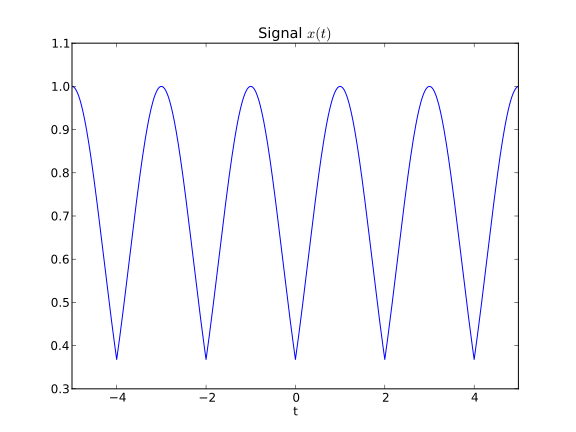
\includegraphics[width=.45\linewidth]{imgs/sig_conv/sig_per.pdf}
    \caption{Examples of causal signal (left) and periodic signal (right).}
    \label{fig:ex_causal_per}
\end{figure}

\paragraph{Signal in $L_p$ space}\index{$L_p$ space}
$L_p(S)$ is the set of functions whose absolute value to the power of $p$
has a finite integral or equivalently that
\begin{equation}
  \|x\|_p=\int_S |x(t)|^p dt < \infty
  \label{eq:lp_space}
\end{equation}
\begin{itemize}
  \item $L_1(\dbR)$ is the set of absolute integrable functions
  \item $L_2(\dbR)$ is the set of quadratically integrable functions (finite energy)
  \item $L_\infty(\dbR)$ is the set of bounded functions
\end{itemize}

\paragraph{Instantaneous power}\index{Power}
The instantaneous power of signal $x(t)$ 
\begin{equation}
  \label{eq:puissinst}
  p_x(t)=|x(t)|^2
\end{equation}
 Unit :  Watt (W).


 \begin{block}{Energy of a signal}\index{Energy}
  We define the energy of a signal $x(t)$ as :
\begin{equation}
\label{eq:enerfinie}
E=\pause \int_{-\infty}^{+\infty}|x(t)|^2dt
\end{equation}
the signal is said to be of finite energy if $E<\infty$ ($\|x\|_2<\infty$ means $x\in L_2(\dbR)$).

Unit: Joule, Calorie or Watt-hour (J, Cal ou Wh, 1 calorie = 4.2 J).
\end{block}

\begin{block}{Average power of a signal}
  
  The average power of a signal is defined as
   \begin{equation}
     \label{eq:puissance}
    P_m= \pause\lim_{T\rightarrow\infty} \frac{1}{T}\int_{-\frac{T}{2}}^{+\frac{T}{2}}|x(t)|^2dt
   \end{equation}
   \begin{itemize}
   \item For a periodic signal, the average power can be computed on a unique period.
   \item Power is homogeneous to an energy divided by time.
   \item $P_{RMS}=\sqrt{P_m}$ is called the Root Mean Square power ("valeur efficace" in french).
   \item A finite energy signal has a n average power $P_m=0$.
   \item  Unit :  Watt (W).
   \end{itemize}
   
     \end{block}


     \begin{block}{Additive noise}
      Additive noise is a kind of noise that is added to the signal of interest.
  $$y(t)=x(t)+b(t)$$
  $y(t)$ is the observed signal, $x(t)$ the signal of interest and
  $b(t)$ is the noise.
    \end{block}

    \begin{block}{Signal-to-Noise ratio (SNR)} \index{SNR}\index{Signal-to-Noise ratio}
      The Signal to Noise Ratio is defined as:
  \begin{equation}
    \label{eq:rsb}
    SNR=\frac{P_S}{P_N} \quad \text{ ou } \quad SNR(dB)=10\log_{10}(SNR)
  \end{equation}
  where $P_S$ is the power of the signal and $P_N$ the power of the noise.
  \begin{itemize}
  \item An Analog-to-Digital conversion process should have the best possible SNR.
  \item The SNR is often used for additive noise models.
  \item Other measures such as Peak Signal to Noise Ratio (PSNR) can be used on specific data (images).
  %\item Le RSB est également appelé SNR pour Signal to Noise Ratio.
  %\item Le Rapport signal sur signal + bruit est également utilisé.
  %$$ R_{S/S+B}=\frac{P_S}{P_{S+B}}$$
  \item One of the objective of filtering is to get a better SNR when the signal and the noise have different frequency contents..
  \end{itemize}
    \end{block}





\subsection{Common signals}
\label{sec:common_sig}


\begin{block}{Heaviside function}
  \begin{equation}
\label{eq:heaviside}
\Gamma(t)=
\begin{cases}
  0& \text{if } t<0\\
  1/2& \text{if } t=0\\
  1 & \text{if } t>0
\end{cases}
\end{equation}
%Exemple: On allume une ampoule.
Also known as the step function. \index{Function!Heaviside}
\end{block}

\begin{block}{Rectangular function}\index{Function!Rectangular}
  \begin{equation}
   \Pi_T (t)=
   \begin{cases}
     1/T& \text{if } |t|< T/2\\
     1/2T& \text{if } |t|= T/2\\
     0& \text{else}
   \end{cases}
   \label{eq:rectangular}
 \end{equation}
 %\vspace{-.5cm}
 \begin{itemize}
 \item $\Pi(t)=\frac{1}{T}(\Gamma(t-\frac{T}{2})-\Gamma(t+\frac{T}{2}))$.
 \item Finite energy signal (finite support).
 \end{itemize}
   \end{block}


   \begin{block}{Complex exponential }\index{Function!Complex exponential}
    let $e_z(t)$ be the following function $\dbR \rightarrow \dbC$
 \begin{equation}
   \label{eq:expcomplexe}
   e_z(t)=\exp(zt)
 \end{equation}
 where $z$ is a complex number.
 When $z=\tau+wi$ the, 
 \begin{equation*}
   \label{eq:expcomplexe2}
   e_z(t)=(\cos(wt)+i\sin(wt))\exp(\tau t)
 \end{equation*}
 %\vspace{5mm}
 
 
 Special cases:
 \begin{itemize}
 \item $z=\tau$ real, then we recover the classical exponential.
 $$e_z(t)=\exp(\tau t)$$
 
 \item $z=wi$ imaginary then
 $$e_z(t)=\cos(wt)+i\sin(wt) $$
 
 % \item $z=\tau+wi$ quelconque alors
 %   $x(t)=(\cos(w*t)+i*\sin(w*t))\exp(\tau t)$
 \end{itemize}
   \end{block}

\begin{figure}[ht]
  \centering
  \begin{tabular}{|c|ccc|}\hline
    $\tau \backslash w$ & $-2$ & $0$ & $2$ \\\hline
   \raisebox{9mm}{$-0.5$} 
    & 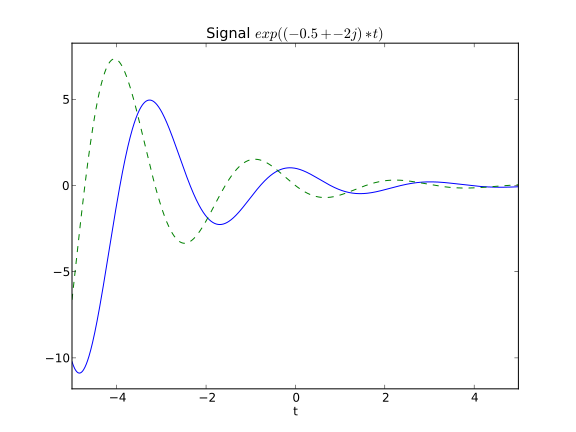
\includegraphics[width=.25\linewidth]{imgs/sig_conv/sig_exp-1-1.pdf}
    & 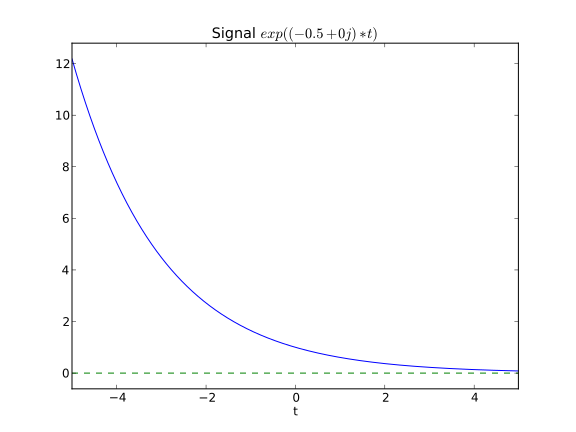
\includegraphics[width=.25\linewidth]{imgs/sig_conv/sig_exp-10.pdf}
    & 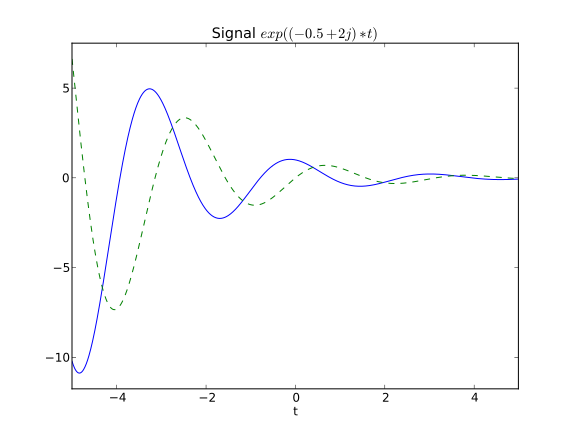
\includegraphics[width=.25\linewidth]{imgs/sig_conv/sig_exp-11.pdf}\\
   \raisebox{9mm}{$0$} 
    & \includegraphics[width=.25\linewidth]{imgs/sig_conv/sig_exp0-1.pdf}
    & \includegraphics[width=.25\linewidth]{imgs/sig_conv/sig_exp00.pdf}
    & 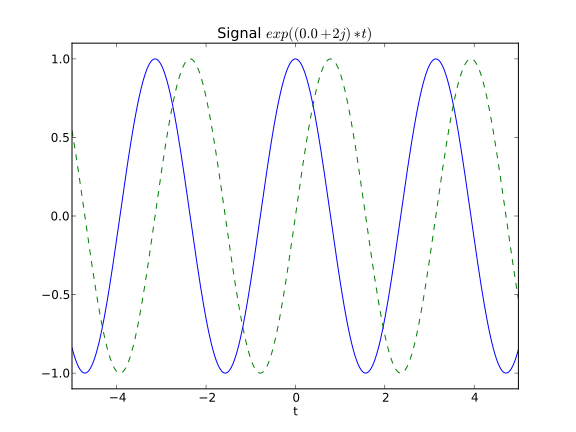
\includegraphics[width=.25\linewidth]{imgs/sig_conv/sig_exp01.pdf}\\
   \raisebox{9mm}{$.5$} 
    & \includegraphics[width=.25\linewidth]{imgs/sig_conv/sig_exp1-1.pdf}
    & \includegraphics[width=.25\linewidth]{imgs/sig_conv/sig_exp10.pdf}
    & 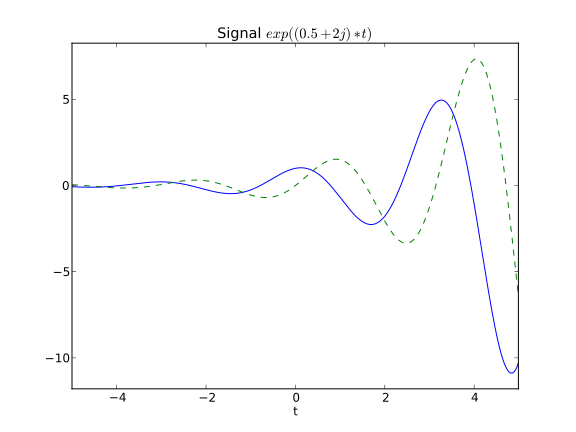
\includegraphics[width=.25\linewidth]{imgs/sig_conv/sig_exp11.pdf}\\
\hline
  \end{tabular}
  \caption{Example of complex exponential for different values of $z$}
  \label{fig:label}
\end{figure}

\subsubsection{Dirac delta}

\index{Dirac delta}
\index{Function!Dirac delta}

\begin{block}{Main properties of Dirac delta}


  \begin{itemize}
    \item Model point mass at $0$.
    \item Value outside $0$ :  $\delta(t)=0, \forall t\neq 0$ 
    %\item Can also be defined as $\lim_{T\rightarrow \infty} \Pi_T(t)$
    \item $\delta$ is a tempered distribution. % (not a function).
    \item Very useful tool in signal processing
   % \item All integrals with $\delta$ will be Lebesgue.
    \item Can be seen as the derivative of the Heavyside function $1_{t\geq 0}(t)$
    \item Integral
    \begin{equation}
      \label{eq:intdirac}
      \int_{-\infty}^{+\infty}\delta(t)dt=1 ,\qquad \int_{-\infty}^{+\infty}x(t)\delta(t)dt=x(0)
    \end{equation}
    \item Dirac and function evaluation for signal $x(t)$ and $t_0\in\R$ :
    %  $$ \delta(t)x(t)=\delta(t)x(0) $$
      $$\delta(t-t_0)x(t)=\delta(t-t_0)x(t_0) $$
   % \item Function evaluation :
    \begin{equation}
      \label{eq:diraceval}
      \langle  x(t) , \delta(t-t_0)\rangle=\int_{-\infty}^{+\infty}x(t)\delta(t-t_0)dt=x(t_0)
    \end{equation}
  
  \end{itemize}
  
  
  \end{block}

  \begin{block}{ Dirac delta definition}

    \begin{itemize}
      \item Let $\phi$ a function supported in $[-1,1]$ of unit mass: $\int_{-\infty}^\infty \phi(u)du=1$ 
      \item  $\phi_T(t)=\frac{1}{T}\phi(\frac{t}{T})$ has support on $[-T,T]$ and unit mass.
      \item We can define the dirac delta $\delta$ as
      $$ \delta(t)=\lim_{T\rightarrow 0} \phi_T(t) $$


    \end{itemize}
    
    
    \end{block}


    \begin{block}{Delta dirac in practice}
      \begin{itemize}
        \item Theoretical object in signal processing (impulse).
        \item Used to model signal sampling for digital signal processing.
        \item Used to model point source  in Astronomy/image processing, point charge in Physics.
        \item Has a bounded discrete variant.
      \end{itemize}
    \end{block}


\frametitle{The dirac comb}\index{Dirac comb}\index{Function!Dirac comb}

\begin{itemize}
  \item The dirac comb is expressed as
  \begin{equation}
    \Sh_T(t)=\sum_{k=-\infty}^\infty \delta(t-kT)
    \label{eq:dirac_comb}
  \end{equation}
  where $\Sh$ is the Cyrilic Sha symbol.
  \item The Fourier Transform of the dirac comb is 
  \begin{equation}
    \mathcal{F}[\Sh_T(t)]=\sum_{k=-\infty}^\infty e^{2i\pi k T f}= \frac{1}{T}\sum_{k=-\infty}^\infty \delta\left(f-\frac{k}{T}\right) =  \frac{1}{T}\Sh_{\frac{1}{T}}(f)
    \label{eq:ft_dirac_comb}
  \end{equation}
  where the second equality comes from the Poisson summation formula.
  \item The dirac comb is used to perform a regular temporal sampling.
  \item Multiplying a signal by the dirac comb corresponds to a convolution by a dirac comb in the Frequency domain (and vice versa).
\end{itemize}
%\end{example}

    \subsection{Discrete time and digital signals}
    \label{sec:}
    

\section{Convolution and filtering}
\label{sec:conv_filtering}

\subsection{Convolution and properties}
\label{sec:}

\index{Convolution}.
\begin{block}{Convolution}
  Let two signals $x(t)$ and $h(t)$. The convolution between the two signals
  is defined as
  \begin{equation}
    x(t)\star h(t) =  \int_{-\infty}^{+\infty}x(\tau)h(t-\tau)d\tau
    \label{eq:convolution}
  \end{equation}\vspace{-5mm}
  \begin{itemize}
    \item Convolution is a bilinear mapping between $x$ and $h$.
    \item It models the relation between the input and the output of a Linear
    Time Invariant system.
    \item If $f\in L_1(\R)$ and $h\in L_p(\R), p\geq1$ then
    $$ \|f\star h\|_p\leq\|f\|_1\|h\|_p $$
    \item The dirac delta $\delta$ is the neutral element for the convolution operator:
\begin{equation}
      \label{eq:dirac_conv}
     x(t)\star \delta(t) =\int_{-\infty}^{+\infty}x(\tau)\delta(t-\tau)d\tau=  x(t)
    \end{equation}
    \begin{equation}
      \label{eq:dirac_conv_tz}
     x(t)\star \delta(t-t_0) = x(t-t_0)
    \end{equation}
 %   $$ x(t) * \delta(t) =  \int_{-\infty}^{+\infty}x(\tau)delta(t-\tau)d\tau=x(t)$$
  \end{itemize}

\end{block}


\paragraph{Example of convolution}
 
% figure in latex, video in HTML
\begin{warpHTML}
  \begin{figure}[ht]
    \centering
    <video width="671" height="472" controls>
    <source src="imgs/sig\_conv/movie\_conv.mp4" type="video/mp4">
    <source src="imgs/sig\_conv/movie\_conv.webm" type="video/webm">
    Your browser does not support the video tag.
    </video>   
    \caption{Illustration of the convolution operator between the Heaviside step function and a causal decreasing exponential.}
    \label{fig:convolution}
  \end{figure}
\end{warpHTML}
\begin{warpprint}
  \begin{figure}[ht]
    \centering
    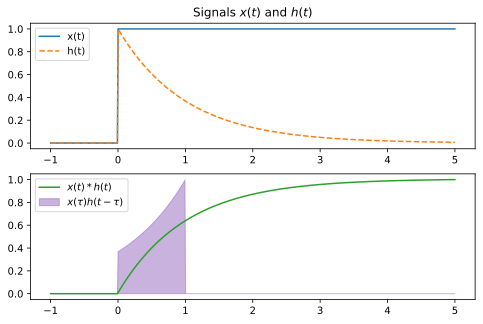
\includegraphics[width=.7\linewidth]{imgs/sig_conv/signals_conv}
    \caption{Illustration of the convolution operator between the Heaviside step function and a causal decreasing exponential.}
    \label{fig:convolution}
  \end{figure}
\end{warpprint}
%\begin{center}
  %\only<1>{ 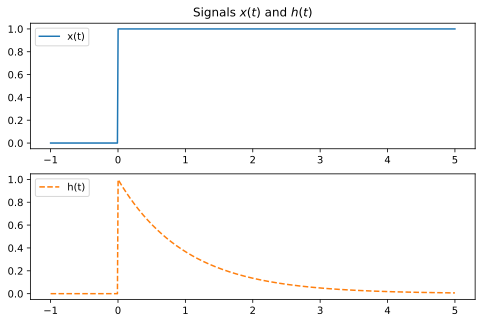
\includegraphics[width=.64\linewidth]{imgs/conv_demo/signals}}

 % \only<2>{ \inlineMovie{imgs/conv_demo/movie.mp4}{imgs/conv_demo/conv_000}{width=.64\linewidth}}
%\only<3>{ \includegraphics[width=.64\linewidth]{imgs/conv_demo/conv_098}}


\begin{itemize}
\item $x(t)=\Gamma(t)$ the Heaviside step function.
\item $h(t)=e^{-t}\Gamma(t)$ the positive part of the decreasing exponential.
\item $x(t)\star h(t)=(1-e^{-t})\Gamma(t)$
\end{itemize}

\subsection{Linear Time Invariant (LTI) systems}
\label{sec:lti_systems}



\begin{block}{Linear Time Invariant (LTI) system}\vspace{-1mm} \index{Linear
Time Invariant system}\index{LTI system}
  \begin{itemize}
  \item A system describes a relation between an input $x(t)$ and an output $y(t)$.
  \item Properties of LTI systems:\vspace{-1mm}
    \begin{itemize}
    \item Linearity \vspace{-3mm}
      $$\quad x_1(t)+ax_2(t)\rightarrow y_1(t)+ay_2(t)$$
    \item Time invariance\vspace{-3mm}
$$x(t-\tau)\rightarrow y(t-\tau)$$
    \end{itemize}
    \item A LTI system can most of the time be expressed as a convolution of the form:
    $$y(t)=x(t)\star h(t)$$
    where $h(t)$ is called the impulse response (the response of the system to an input $x(t)=\delta(t)$)
  \end{itemize}
\end{block}


\begin{exampleblock}{Examples}
\begin{itemize}
\item Passive electronic systems (resistor/capacitor/inductor) .
\item Newtonian mechanics, Fluid mechanics, Fourier Optics.
\end{itemize}
\end{exampleblock}



\begin{block}{Ordinary Differential Equation (ODE)} \index{Ordinary Differential Equation}
  The system is defined by a linear equation of the form:
  \begin{equation}
    \label{eq:edo}
    a_0y(t)+a_1\frac{dy(t)}{dt}+\dots+a_n\frac{d^ny(t)}{dt^n}=
    b_0x(t)+b_1\frac{dx(t)}{dt} +\dots+b_m\frac{d^mx(t)}{dt^m}
  \end{equation}
  
  \begin{itemize}
  \item ODE based system with linear relations are an important class of LTI systems.
  \item Also called homogeneous linear differential equation.
  %\item $\max(m,n)$ est l'ordre du système.
  %\item Également appelées équations différentielles linéaires à coefficients
  %constants.
  \item $n$ is the number of derivatives for $y(t)$ and $m$ for $x(t)$.
  \item $\max(m,n)$ is the order of the system.
  \item The output of the system can be computed from the input by solving Eq.
    \eqref{eq:edo}.
    \item Linearity and time invariance are obvious from equation.
  \end{itemize}
  
  \end{block}


\section{Discrete time and digital signals}
\label{sec:def_discrete_signal}

\subsection{Discrete time}

  \index{Discrete time!Definition}
\begin{block}{Notations}
  \begin{itemize}
      \item $x(t)$ with $t\in\R$ is the analog signal.
      \item $x_T(t)$ with $t\in\R$ is the sampled signal of period (T) but still continuous time:
      $$  x_T(t)=\sum_{n=-\infty}^\infty x(nT)\delta(t-nT) $$
      \item $x[n]$ with $n\in\mathbb{Z}$ is the discrete signal sampled with period $T$ such that:
      $$  x[n]= x(nT) $$
      \item Obviously one can recover $x_T(t)$ from $x[n]$ with
      $$  x_T(t)=\sum_{n=-\infty}^\infty x[n]\delta(t-nT) $$
      \item In order to simplify notations we will suppose $T=1$ in the following.
      \item In this course we suppose that $|x[n]|$ is bounded.
  \end{itemize}
\end{block}


\begin{center}
  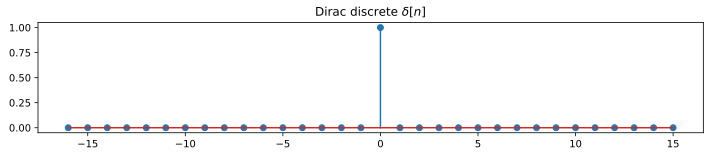
\includegraphics[width=.8\linewidth]{imgs/sig_conv/dirac_delta_discrete}
\end{center}\vspace{-5mm}

\index{Discrete time!Dirac Delta}\index{Dirac delta}
\begin{block}{Discrete dirac}
  We note the discrete dirac $\delta[n]$ defined as\vspace{-2mm}
  \begin{equation}
      \delta[n]=
      \begin{cases}
          1& \text{for } n=0\\
          0 & \text{else}
        \end{cases}
      \label{eq:discrete_dirac}
  \end{equation}\vspace{-5mm}
\end{block}

\begin{block}{Discrete signal}\index{Discrete time!Signal}
  Any discrete signal $x[n]$ can be decomposed as a sum of translated discrete diracs:\vspace{-1mm}
  \begin{equation}
      x[n]=\sum_{k=-\infty}^\infty x[k]\delta[n-k]
      \label{eq:discreet_signal_dirac}
  \end{equation}\vspace{-2mm}

  The discrete diracs are an orthogonal basis of $L_2(\mathbb{Z})$ of scalar product and corresponding norm  \vspace{-2mm}$$<x[n],h[n]>=\sum_{k=-\infty}^\infty x[k]h^*[k],\qquad \|x[n]\|^2=<x[n],x[n]>=\sum_{k=-\infty}^\infty |x[k]|^2.$$ 
\end{block}


\begin{block}{Convolution between discrete signals}\index{Discrete
time!Convolution}\index{Discrete convolution}\index{Digital filtering!Convolution}
  Let $x[n]$ and $h[n]$ two discrete signals. The convolution between them is expressed as:
  \begin{equation}
      x[n]\star h[n]= \sum_{k=-\infty}^\infty x[k]h[n-k]
      \label{eq:discrete_convolution}
  \end{equation}

\end{block}

\begin{block}{Digital filter properties}\index{Digital filtering!Properties}
  Let the discrete system/operator/filter $L$ described by its impulse response $h[n]$.
  \begin{itemize}
      \item \textbf{Causality} $L$ is causal if $h[n]=0,\ \forall n\leq 0$. $L$ is causal if 
   \begin{equation}
          h[n]=h[n]\Gamma[n],\qquad\text{where}\qquad     \Gamma[n]=
          \begin{cases}
              1& \text{for } n\geq 0\\
              0 & \text{else}
            \end{cases}
          \label{eq:causal_discrete}
      \end{equation}
      \item \textbf{Stability} A system is stable if the output of a bonded input is bounded. A necessary and sufficient condition is that
      \begin{equation}
          \sum_{n=-\infty}^\infty |h[n]|<\infty
          \label{eq:stable_system}
      \end{equation}
      
      
  \end{itemize}
  
\end{block}

\subsection{Finite signals}
\label{sec:finite}

\index{Finite signals}

\begin{center}
  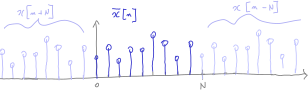
\includegraphics[width=.8\linewidth]{imgs/sig_conv/finite_discrete-crop.pdf}
\end{center}

\begin{block}{Finite discrete signals}\index{Discrete time!Finite Signal}
  \begin{itemize}
      \item Most of the theoretical results seen up to now correspond to signals $x[n]$ where $n\in\mathbb{Z}$.
      \item In practice recordings are only done for a finite amount of time resulting to only $N$ samples. 
      \item We defined $\tilde x[n]$ a finite signal of $N$ samples with $n\in \{0,\dots,N-1\}$.
      \item We use in the following the periodization of $\bar x[n]$
      $$ x[n] = \tilde x[n\mod N] $$
      where $\mod$ is the modulo operator.
  \end{itemize}
\end{block}

\begin{block}{Discrete convolution of finite signals}\index{Discrete time!Convolution}\index{Discrete convolution}
  The convolution between $\tilde x[n]$ and $\tilde h[n]$ both finite signals of $n$ samples can be expressed as:
  \begin{equation}
      \tilde y[n]=\tilde x[n]\star\tilde h[n] =  \sum_{p=-\infty}^{+\infty}
      \tilde x[p] \tilde h[n-p] 
      \label{eq:conv_finite}\vspace{-3mm}
  \end{equation}
  \begin{itemize}
      \item It requires values for the signals outside of the sampling widow. 
      \item One common approach consists in having $\tilde x[n]$ and $\tilde h[n]$ equal to $0$ outside the sampling interval. Other choices can be done (see next slides)
 %     \item In this case only the center sample is exact.
  \end{itemize}
\end{block}

\begin{block}{Circular convolution}\index{Discrete time!Circular convolution}\index{Circular convolution}
  When using the periodic version of the signals the circular convolution can be computed on a unique period of size $N$:
  \[
      x \ostar h [n] 
      = \sum_{p=0}^{N-1}
      x[p] h[n-p] .
      \] 
The circular convolution is rarely appropriate in real life images due to border effects.
 % Note that thanks to the 
\end{block}

\begin{block}{Vector representation and convolution
matrix}\vspace{-2mm}\index{Convolution matrix}
  \begin{itemize}
      \item Finite signal $x$ of $N$ samples can be represented as a vector $\x\in\mathbb{C}^N$.
      \item The convolution operator is linear and can be expressed as:\vspace{-1mm}
      $$ \y=\x\star\h= \C_\h \x $$
      Where\vspace{-1mm} $\C_\h\in \mathcal{M}_\mathbb{C}(N,N)$ is a convolution matrix parametrized by vector $\h$.
  \end{itemize} \vspace{-4mm}
\end{block} %\vspace{-5mm}

\begin{block}{Discrete convolution}\index{Discrete convolution}
  The convolution operator when the values outside the support are $0$ can be expressed as\vspace{-2mm}
  $$ \hspace{-3mm}\C_\h\hspace{-.5mm} =\hspace{-.5mm}\begin{bmatrix}
      h[0] & 0 & \cdots& 0\\
      h[1] & h[0] & \cdots& 0\\
      \vdots & \vdots & \ddots & \vdots\\
      h[N\hspace{-.5mm}-\hspace{-.5mm}1] & h[N\hspace{-.5mm}-\hspace{-.5mm}2 ] & \dots&  h[0]\\
      \vdots & \vdots & \ddots & \vdots\\
      0 & 0 &\cdots & h[N\hspace{-.5mm}-\hspace{-.5mm}1] 
  \end{bmatrix} $$
  where $\C_\h\in \mathcal{M}_\mathbb{C}(2*N-1,N)$ is a Toeplitz matrix.
\end{block}

\begin{block}{Circular convolution}\index{Circular convolution}
  The circular convolution operator can be expressed as
  $$ \C_\h =\begin{bmatrix}
      h[0] & h[N-1] & \cdots& h[1]\\
      h[1] & h[0] & \cdots& h[2]\\
      \vdots & \vdots & \ddots & \vdots\\
      h[N-1] & h[N-2 ] & \dots&  h[0]\\
  \end{bmatrix} $$
  where $\C_\h\in \mathcal{M}_\mathbb{C}(N,N)$ is a circulant Toeplitz matrix.
\end{block}

\begin{center}
  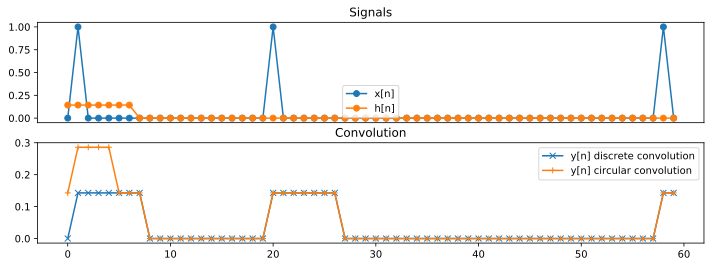
\includegraphics[width=.9\linewidth]{imgs/sig_conv/circ_conv_border.pdf}
\end{center}

\begin{itemize}
  \item Convolution between diracs $\tilde x[n]$ and a shape $h[n]$ will repeat the shape at the diracs position.
  \item A dirac at the end of the signal will cut the shape for discrete convolution where the outside of the sampling is $0$.
  \item With circular convolution the shape is repeated t the beginning of the signal.
  \item One can remove border effects by creating virtual periodic signal with zeros (zero padding, see fast convolution).
\end{itemize}



\begin{center}
  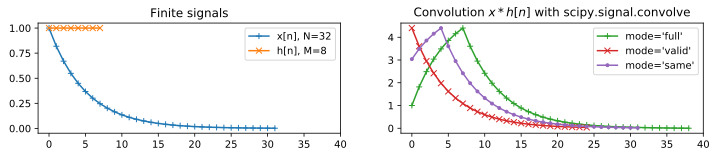
\includegraphics[width=1\linewidth]{imgs/sig_conv/conv_scipy_signal.pdf}
\end{center}\vspace{-2mm}

\begin{block}{The Scipy \incode{scipy.signal.convolve} function:}\vspace{-2mm}
  \begin{itemize} \index{Python!\incode{scipy.signal.convolve}}
      \item Convolution between two signals of support respectively $N$ and $M$ samples supposing that their values are $0$ outside of the support.
      \item The third parameter is \incode{mode} that change the size of the output : \vspace{-1mm}
      \begin{itemize}
          \item \incode{mode='full'} returns a signal of support $N+M-1$ (default).
          \item \incode{mode='valid'} returns a signal of support $|N-M|+1$ with only  the samples that do not rely on zeros padding of the larger signal.
          \item \incode{mode='same'} returns a signal of the same size as the first input.
      \end{itemize}
      \item Parameter \incode{method} allows to choose between \incode{'direct'} computation and \incode{'fft'} and selects the most efficient by default.
  \end{itemize}
  

  
\end{block}\vspace{-2mm}


\begin{center}
  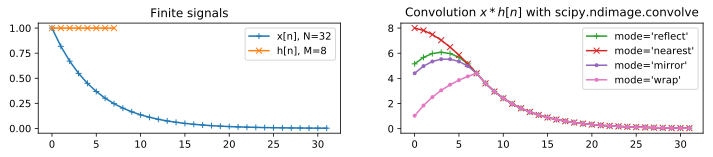
\includegraphics[width=1\linewidth]{imgs/sig_conv/conv_scipy_ndimage.pdf}

\end{center}\vspace{-2mm}

\begin{block}{The Scipy \incode{scipy.ndimage.convolve}  function:}\vspace{-2mm}
  \begin{itemize}\index{Python!\incode{scipy.ndimage.convolve}}
      \item Always return the same size as the first parameter by default.
      \item  The \incode{mode} parameter allows selecting the borders of a signal $x=(abcd)$:
      \begin{itemize}
          \item \incode{mode='reflect'} : $(d c b a | a b c d | d c b a)$ (default)
          \item  \incode{mode='constant'} : $(k k k k | a b c d | k k k k)$
          \item \incode{mode='nearest'} : $(a a a a | a b c d | d d d d)$
          \item \incode{mode='mirror'} : $(d c b | a b c d | c b a)$
          \item \incode{mode='wrap'} : $(a b c d | a b c d | a b c d)$ (circular convolution)
      \end{itemize}
      \item  Parameter \incode{origin} allows to select the origin of the filter $h$.
  \end{itemize}
  


\end{block}


\subsection{Quantization and storage}
\label{sec:}

\index{Quantization}

\section{Fundamental signal processing problems}
\label{sec:sp_prob}

\subsection{Filtering}

\index{Filtering}


\subsection{Deconvolution, unmixing and regression}

\index{Deconvolution}

\index{Inverse problem}


\subsection{Blind source separation and deconvolution}

\index{Blind source separation}





\chapter{Fourier analysis and analog filtering}
\label{chap:fourier-analog}



  \begin{itemize}
    \item A signal is $x(t)$ a function of time, an image $x(\v)$ a function of space.
    \item Those functions are what we measure/observe  but can be hard to
    interpret/process automatically.
    \item Another representation for a signal is in the frequency domain ($1/t$).
    \item Better representation for numerous applications.
  \end{itemize}


  \begin{exampleblock}{Applications}
    \begin{itemize}
      \item Signal processing (biomedical, electrical).
      \item Image processing (2D signals), filtering, reconstruction.
      \item Colors are combination of waves of different frequencies.
    \end{itemize}
  \end{exampleblock}
  
\section{Fourier series}
\label{sec:fourier-transform}

\index{Fourier series}

\begin{center}
    \includegraphics[width=.7\linewidth]{imgs/fourier/fourier_series_title}
    \includegraphics[width=.2\linewidth]{imgs/fourier/fourier}

    \includegraphics[width=.7\linewidth]{imgs/fourier/fourier_series1}
    \includegraphics[width=.7\linewidth]{imgs/fourier/fourier_series2}
  \end{center}
  \vspace{-5mm}
  \begin{block}{History}
    \begin{itemize}
      \item Trigonometric series used by Euler, d'Alembert, Bernoulli and Gauss.
      \item Introduced by Joseph Fourier in \cite{fourier1807memoire}.
      \item Fourier claimed that these series could approximate any function.
    \end{itemize}

  \end{block}


  \begin{block}{Decomposition as trigonometric series}
    One can express periodic $x(t)$ of period $T_0=\frac{2\pi}{w_0}$ integrable on the period as
$$
x(t)= \frac{a_0}{2} + \sum_{k=1}^\infty \left [a_k \cos (k w_0 t) +
  b_k \sin (k w_0 t) \right]
$$

where $a_k$ and $b_k$ are the Fourier coefficients that can be computed as
$$
a_k = \frac{2}{T_0} \int_{T_0} x(t) \cos (k w_0 t) dt \quad \quad b_k
= \frac{2}{T_0} \int_{T_0} x(t) \sin (k w_0 t) dt
$$

\begin{itemize}
  \item Representation of a periodic signal as an infinite number of coefficients corresponding to harmonic frequencies.
  \item Can be interpreted as a change of basis from temporal to frequencies.
  \item Functions can be approximated with a finite number $N$ of terms.
  \item Gibbs phenomenon appears for discontinuous functions \cite{hewitt1979gibbs}.
\end{itemize}

\end{block}


\begin{figure}[t]
    \centering
    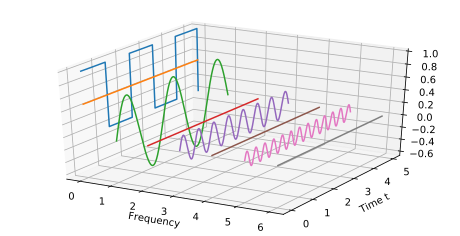
\includegraphics[width=.64\linewidth]{imgs/fourier/fourier_series_3d}
    \caption{Illustration of Fourier series for Example }
    \label{fig:label}
\end{figure}

\begin{exampleblock}{Example : Square wave}
    \begin{columns}
      \begin{column}{5cm}
        \begin{itemize}
        \item Square wave with $T_0=2$
  %$$x(t)=\sum_{k=-\infty}^\infty \Pi_T(t-\frac{T}{2}-kT)$$

      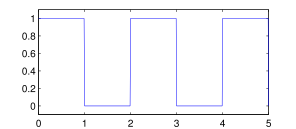
\includegraphics[width=.5\columnwidth]{imgs/fourier/sig_creneau}
        \end{itemize}
      \end{column}
      \begin{column}{6cm}
        \begin{itemize}
        \item $x(t)=\sum_{i=-\infty}^\infty 1_{[iT_0,iT_0+T_0/2 ]}(t)$
        \item $a_0=1, a_k=0 \quad \forall k >0$
        \item $b_k=\frac{2}{\pi k}$ for $k$ odd else $b_k=0$
        \end{itemize}
      \end{column}
    \end{columns}
  \end{exampleblock}

    
 \begin{block}{Complex harmonic decomposition}
    One can express periodic $x(t)$ of period $T_0=\frac{2\pi}{w_0}$ integrable on the period as
  $$
  x(t) = \sum_{k=-\infty}^{^\infty}  c_k  e^{jkw_0t} \quad \quad \text{ avec }
  w_0= \frac{2 \pi }{T_0}
  $$
  where the coefficients $c_k$ are called the  \textbf{complex Fourier coefficients} and can be computed with
  $$
  c_k = \frac{1}{T_0} \int_{T_0} x(t) e^{-j k w_0t}dt = \frac{1}{T_0} \int_{0}^{T_0} x(t) e^{-j k w_0t}dt = \frac{1}{T_0} \int_{-T_0/2}^{T_0/2} x(t) e^{-j k w_0t}dt
  $$
    \end{block}
  \vspace{-5mm}
    \begin{block}{Relations between decompositions}
     Using the Euler formula we can show that $a_k$ and $b_k$ and the $c_k$ coefficients are related by
  $$
  \frac{a_0}{2}= c_0 \quad \quad a_k = c_k + c_{-k} \quad \quad b_k =
  j(c_k - c_{-k})
  $$
  % et
  % $$
  % c_k=\frac{a_k -j b_k}{2} \quad \quad c_{-k}=\frac{a_k +j b_k}{2}
  % $$
  
  Note that if $x(t)$ is an even function then the
  $b_k=0$ , and if $x(t)$ is odd then $a_k=0$.
    \end{block}

  %\lipsum[2-4]
\section{Fourier transform}
\label{sec:fourier-transform}


\subsection{Definition}
\label{sec:}

    The Fourier Transform (FT) of a signal  $x(t)$ can be expressed as
    \index{Fourier transform}\index{Fourier transform!Definition}

    \begin{equation}
      \mathcal{F}[x(t)]= X(f) = \int_{-\infty}^\infty e^{- i 2 \pi f t} x(t) d t 
      \label{eq:fourier_tranform}
    \end{equation}
    When it exists the inverse Fourier transform is defined as
    \begin{equation}
      \mathcal{F}^{-1}[X(f)] = x(t)= \int_{-\infty}^\infty e^{  2 i  \pi f t} X(f) d f
      \label{eq:inverse_fourier}
    \end{equation}

    \begin{itemize}
      \item Note that the $\hat \;$ operator is also often used for the Fourier
      transform $\hat x$ of $x$.
      \item In signal processing the references often use $j$ instead of $i$
      for the imaginary number ($i$ is a measure of current).
      % \item The FT relations are denoted in this course as follows:
      % $$
      % x(t) \rightleftharpoons X(f)
      % $$
      \item The FT is a change of representation for the function $x$ from the temporal representation to the harmonic (frequency) representation.
   %   \item Existence of the inverse Fourier transform is complex and discussed later.
    \end{itemize}

    % \begin{align}
    % \label{eq:TFL1}
    % &[\TFA{f}](\xi)= \hat{f}(\xi) = \int_{\rset} \rme^{- \rmi 2 \pi \xi x} f(x) \rmd x \\
    % &[\TFAC{f}](x) = \int_{\rset} \rme^{ \rmi 2 \pi \xi x} \hat{f}(\xi) \rmd x
    % \end{align}
    % On appelle $\TFA{f}$ (not{\'e} aussi $\TF f$) la \emph{Transform{\'e}e de Fourier} de $f$ et $\TFAC{f}$  (not{\'e} aussi $\TFC f$) la
    % transform{\'e}e de Fourier conjugu{\'e}e de $f$.



    $$
    x(t)= \int_{-\infty}^\infty \rme^{ \rmi 2 \pi f t} X(f) \rmd f
  $$

  \begin{block}{Harmonic representation}
    \begin{itemize}
    \item The FT represents the signal in the frequency domain.
    \item $|X(f)| $ is the magnitude of a sinusoidal signal for frequency $f$.
\item $Arg(X(f)$ is the phase of the sinusoidal signal.
    \item For a real signal $x(t)$, $X(f)=X(-f)^*$ and an informal interpretation would be
      \begin{align}
        x(t) &= \int_{-\infty}^{+\infty} X(f) e^{i2\pi f t} df= \int_{-\infty}^{+\infty} |X(f)| e^{i2\pi (f t+Arg(X(f)))} df\\
        &\approx X(0)+2
        \int_{0+}^{+\infty} |X(f)| \cos(2\pi (f t+Arg(X(f))) )\label{eq:1}
      \end{align}
    \item The modulus and argument of the FT allow identification of the frequency content of the signal and its phase.
   % \item This representation allows for simple interpretation of 
    \end{itemize}
  \end{block}


  \paragraph{Fourier Transform in $L_p(\R)$}



  \begin{itemize}
    \item For $1 \leq p \leq 2 $ the FT maps from $L_p(\R)$ to
    $L_q(\R)$ with $\frac{1}{p}+\frac{1}{q}=1$.
    \item Consequence of the Riesz–Thorin theorem.
      \item The TF of an absolute integrable function is bounded (Example : rectangle).
   %   \item The TF of a bounded function is absolute integrable.
   %   \item T
  \end{itemize} \vspace{-3mm}
  
  
  \begin{block}{Parseval-Plancherel identity in $L_2$}
    The TF of an $L_2$ function is $L_2$. Note that  $L_2$ is a Hilbert
      space of inner product:
      $$ <x,y> = \int_{-\infty}^\infty x(t)y^*(t)dt$$
    For two functions $x,y\in L_2(\R)^2$ of respective TF $X,Y\in L_2(\R)^2$  the
    Parseval-Plancherel identity states that
    \begin{equation}
      <x,y> =  \int_{-\infty}^\infty x(t)y^*(t)dt= \int_{-\infty}^\infty X(f)Y^*(f)df
      \label{eq:parseval}
    \end{equation}
\begin{equation}
    <x,x> = \int_{-\infty}^\infty |x(t)|^2dt= \int_{-\infty}^\infty |X(f)|^2df
        \label{eq:parseval2}
\end{equation}
      which means that the energy of a signal is preserved by FT.
  
  
  \end{block}
  
  More details in \cite[Chap. 5.A]{hunter2019notes} and \cite[Chap. 1]{mallat2015traitement}


  \frametitle{Fourier Transform in $\R^d$}\index{Fourier transform! Fourier
  transform in $\R^d$}

  The Fourier Transform can be naturally extended to functions in $\R^d$.

  \begin{block}{Fourier Tansform in $\R^d$}
    Let $x(\v): \R^d \rightarrow \mathbb{C}$, the Fourier Transform of $x$ can be expressed as 
    \begin{equation}
      \mathcal{F}[x(\v)]= X(\u) = \int_{\R^d} x(\v) e^{-2i\pi <\v,\u>} \rmd \v 
      \label{eq:fourier_tranform_rd}
    \end{equation}
    When it exists the Inverse FT is defined as
    \begin{equation}
      \mathcal{F}^{-1}[ X(\u)]= x(\v) = \int_{\R^d} X(\u) e^{2i\pi <\v,\u>} \rmd \u 
      \label{eq:in_fourier_tranform_rd}
    \end{equation}\vspace{-2mm}
    \begin{itemize}
      \item $\u \in \R^d$ is a directional frequency. 
      \item All the properties of the 1D FT are preserved (duality, convolution, ...)
      \item With $d=2$, frequency representation of black and white images.
      \item With large $d$, approximation for efficient kernel approximation in machine learning \cite{rahimi2008random}.
    \end{itemize}
  \end{block}

  \frametitle{Fourier transform and angular
  frequency}\index{Frequency}\index{Angular frequency}
  \begin{itemize}
  \item The FT in this course is a function of frequency $f$ (in Hz).
  \item Another common way to represent frequency is the angular frequency $w$ (in rad/s) such that
%  \item Frequency and angular frequency are related with
$$w=2\pi f,\quad \quad\quad f=\frac{w}{2\pi}$$
\item When using angular frequency the FT is non-unitary meaning that :
 $$   \mathcal{\tilde F}[x(t)]= \tilde X(w) = \int_{-\infty}^\infty \rme^{- \rmi w t} x(t) \rmd t  $$
 $$   \mathcal{\tilde F}^{-1}[X(f)] = x(t)= \frac{1}{2\pi}\int_{-\infty}^\infty \rme^{ \rmi w t} \tilde X(w) \rmd w $$
 \item There exists a unitary angular frequency FT that scales both FT and IFT by $\frac{1}{\sqrt{2\pi}}$.
  \item In the following we will sometime use the FT as a function of the angular frequency:
  $$ \tilde X(w)=X\left(\frac{w}{2\pi}\right)$$

 % \item This is a change of variable in the function but not a FT with $w$ !
  \end{itemize}

  \subsection{Examples of Fourier Transform}
  \label{sec:}
\index{Fourier transform!Examples}
  \begin{exampleblock}{Rectangular function}
    %\vspace{5mm}
      \begin{columns}
          \begin{column}%{.5\linewidth}
     \begin{equation}
      \label{eq:echelon}
      \Pi_T(t)=
      \begin{cases}
        1/T& \text{if } |t|< T/2\\
        1/2T& \text{if }  |t|= T/2\\
        0& \text{else}
      \end{cases}
    \end{equation}
    
      The Fourier transform is
      \begin{align*}
        \mathcal{F}[\Pi_T(t)]=&   \frac{1}{T}\int_{-T/2}^{T/2} e^{- i 2 \pi f t} \rmd t \\
        =& \left[\frac{-\rme^{- \rmi 2 \pi f t}}{\rmi 2 \pi fT}\right]_{-T/2}^{T/2}\\
        =&  \frac{\rme^{\rmi \pi f T}-\rme^{- \rmi \pi f T}}{\rmi 2 \pi fT}\\
        =& {\frac{\sin(\pi f T)}{\pi f T} = \text{sinc}(\pi f T)}
      \end{align*} 
    % $$
    % \mathcal{F}[\Pi_T(t)]= \beamer{\frac{\sin(\pi f T)}{\pi f T} = \text{sinc}(\pi f T)}
    % $$
    with 
    $\text{sinc}(t)= \frac{\sin(t)}{t}\quad\text{ and } \text{sinc}(0)=1$

          \end{column}
          \begin{column}%{.4\linewidth}
            \begin{center}
            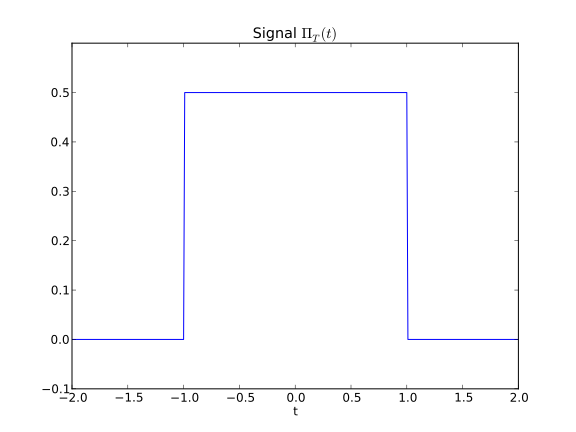
\includegraphics[width=.45\columnwidth]{imgs/fourier/sig_porte_ft.pdf}
            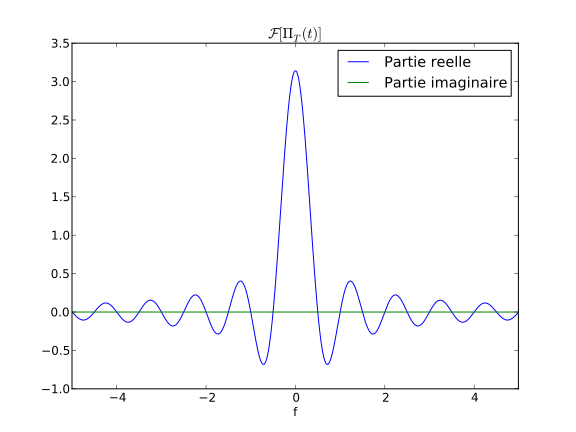
\includegraphics[width=.45\columnwidth]{imgs/fourier/ft_sig_porte_ft.pdf}
          \end{center}
         \end{column}
        \end{columns}
    
    
      \end{exampleblock}


      \begin{exampleblock}{Decreasing exponential}
        \vspace{-5mm}
          \begin{columns}
              \begin{column}%{.5\linewidth}
        $$x(t) = e^{-at} \Gamma(t), \quad   \Gamma(t)=
        \begin{cases}
          1& \text{for } t>0\\
          1/2& \text{for } t=0\\
          0& \text{else}
        \end{cases}$$
        with $a>0$
        
        The Fourier transform is
        \begin{align*}
          \mathcal{F}[e^{-at} \Gamma(t)]=&  \int_{0}^\infty e^{-at} \rme^{- \rmi 2 \pi f t}  dt\\
          =&  \int_{0}^\infty e^{-(a+ \rmi 2 \pi f)t} dt\\
          =& \left[\frac{\rme^{-(a+ \rmi 2 \pi f)t}}{-(a+ \rmi 2 \pi f)}\right]_0^\infty\\
          =&\frac{1}{a+ i 2 \pi f}
        \end{align*}
        % $$
        % X(f)= \beamer{\frac{1}{a+ j 2 \pi f}}
        % $$
               \end{column}
              \begin{column}%{.4\linewidth}
                \begin{center}
                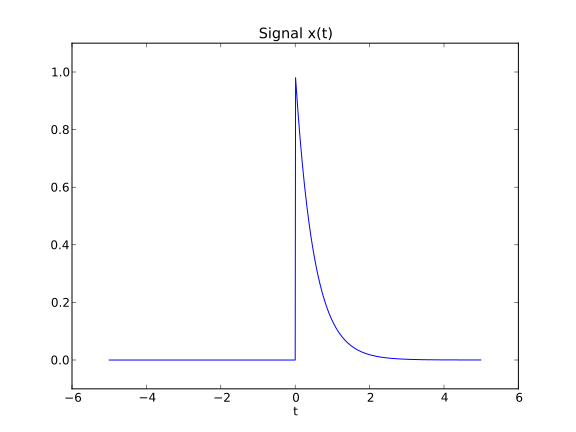
\includegraphics[width=.45\columnwidth]{imgs/fourier/sig_exp_ft.pdf}
                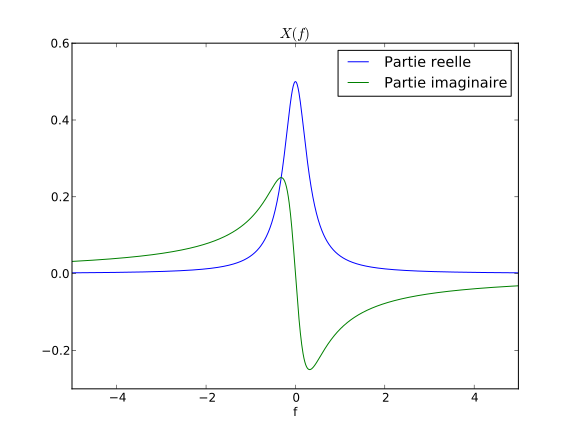
\includegraphics[width=.45\columnwidth]{imgs/fourier/ft_sig_exp_ft.pdf}
              \end{center}
             \end{column}
            \end{columns}
        
          \end{exampleblock}


\subsection{Properties of the Fourier Transform}
\label{sec:}\index{Fourier transform!Properties}

\begin{block}{Linearity}\index{Properties!Linearity}
    Ley $x_1(t)$ and $x_2(t)$ two signals of TF $X_1(f)$ and $X_2(f)$ respectively. 
  
  For $a \in \R$ and $b \in \R$, we have :
  
  $$
  \mathcal{F}[a x_1(t) + b x_2(t)]=  a X_1(f) + b X_2(f)
  $$
  
  %\begin{demo}
    Comes from the linearity of the integration.
 % \end{demo}
  \end{block}
  
  
  \begin{block}{Time shift}\index{Time shift}
    Let $x(t)$ be a signal of FT $X(f)$. 
  
  For $t_0 \in \R$, let $x(t-t_0)$ a time shift of  $x(t)$ then we have:
  $$
  \mathcal{F}[x(t-t_0)]= e^{-i 2 \pi t_0f}X(f)
  $$
  %\begin{demo} 
    Change of variable in the integral.
  %\end{demo}
  \end{block}
  

  


  \begin{block}{Frequency shift}\index{Frequency shift}

    Let $x(t)$ be a signal of FT $X(f)$ then we have 
  $$
  \mathcal{F}\left[e^{i 2 \pi f_0t} x(t) \right]= X(f-f_0)
  $$
  Multiplication by a complex exponential of frequency $f_0$, translates the TF by
  $f_0$.
  
  %\begin{demo}
     Regroup exponentials in the integral.
  %\end{demo}
\end{block}


\begin{block}{Time scaling}\index{Time scaling}
  Let $x(t)$ be a signal of FT $X(f)$  and $a$ a scaling $a \neq 0$ then we have
$$
\mathcal{F}[x(at)]= \frac{1}{|a|} X\left(\frac{f}{a}\right)
$$
%\begin{demo} 
    Change of variable for separate cases $a>0$ and $a < 0$.
%\end{demo}
\end{block}




\begin{block}{Derivation}\index{Fourier Transform!Derivative}
    Let $x(t)$ be a signal of FT $X(f)$ then we have 
  $$
  \mathcal{F}\left[\frac{d x(t)}{ dt }\right]=  i 2 \pi f X(f)
  $$
  % \begin{demo} Dériver le deux termes définissant la
  %   transformée de Fourier par $t$.
  % \end{demo}
  \end{block}
  
  
  \begin{block}{Integration}
    Let $x(t)$ be a signal of FT $X(f)$ such that
    $\int_{-\infty}^\infty x(t) dt = 0$ then we have
  $$
  \mathcal{F}\left[\int_{-\infty}^t x(u) du \right]= \frac{1}{i 2 \pi f }  X(f)
  $$
  If   $\int_{-\infty}^\infty (x(t)-c) dt = 0$ where $c$ is often called the constant term, we have
  $$
  \mathcal{F}\left[\int_{-\infty}^t x(u) du \right]= \frac{1}{i 2 \pi f }  X(f)+ c\delta(f)
  $$
  where $\delta(f)$ is the Dirac delta.
  \end{block}

  Those two properties can be used to solve Ordinary Differential Equations
  (ODE).
  


\begin{block}{Even and odd signals}\index{Properties!Even and odd signals}
    \begin{center}
      \begin{tabular}{|l|l|}
        \hline
        $x(t)$ & $X(f)$\\ \hline
        Even real & Even real \\
        Odd real & Odd imaginary \\
        Even imaginary & Even imaginary\\
        Odd imaginary & Odd real\\ \hline
      \end{tabular}
    
      
    \end{center}
    For a real signal $x(t)$ : $X(f)=X(-f)^*$ 
    \end{block}
      % \begin{itemize}
      % \item Si un signal $x(t)$ est un signal réel et pair alors $X(f)$
      %   est réelle et paire.
    
    
      % \item Si un signal $x(t)$ est un signal réel impair alors $X(f)$ est
      %   imaginaire pure et impaire.
      % \end{itemize}
    
    
    
    \begin{block}{Conjugate signal}
      Let $x(t)$  be a signal of FT $X(f)$ and
      $x^*(t)$ its complex conjugate, then we have
    $$
    \mathcal{F}[x^*(t)] = X^*(-f)
    $$
    \end{block}


    \paragraph{Duality of the Fourier Transform}\index{Fourier transform!Duality}
    

Let $x(t)$ be a signal of FT $X(f)$. 
% Par définition, on a
% $$
% X(f)= \int_{-\infty}^{+\infty} x(t) e^{-j2 \pi f t} dt 
% $$
% et la définition de la transformée inverse donne
% $$
% x(t)= \int_{-\infty}^{+\infty} X(f) e^{j2 \pi f t} df
% $$
% De par cette dernière définition
When the inverse Fourier transform exists we can write
$$
x(-t)= \int_{-\infty}^{+\infty} X(f) e^{j2 \pi f (-t) } 
df = \int_{-\infty}^{+\infty} X(f) e^{-j2 \pi f t } 
df 
$$

\begin{itemize}
  \item The last term is the TF of function $X(f)$.
  \item This means that if $ \mathcal{F}[x(t)]=X(f)$ then
  $$ \mathcal{F}[X(t)]= x(-f)$$
  \item Applying twice the TF operator to $x(t)$ returns $x(-t)$: 
  \ $ \mathcal{F}[\mathcal{F}[x(t)]]=x(-t)$
\end{itemize}

% Le dernier terme de l'égalité correspond à la transformée
% de Fourier de la fonction $X(f)$. En intervertissant
% les variables temporelles $t$ et les variables
% fréquentielles $f$, on a donc
% si 
% $
% x(t) \rightarrow X(f)
% $ alors

% $$
% X(t) \rightarrow x(-f)$$


%\begin{example}
     For the rectangular function $ \Pi_T(t)$ : 

$$
\begin{array}{l}
  \Pi_T(t) \rightarrow  \text{sinc}(\pi f T) \\
  \text{sinc}(\pi T t )\rightarrow {\Pi_T(-f) =\pause \Pi_T(f)}
\end{array}
$$


\paragraph{Convolution and Fourier Transform}\index{Fourier transform!Convolution}\index{Convolution}
\begin{block}{Convolution and Fourier Transform}
  Let two signals $x(t)$ and $h(t)$ of respective Fourier transform $X(f)$ and
  $H(f)$ then 
  \begin{equation}
    \mathcal{F}
    [ x(t)\star h(t)]  = X(f)H(f)
    \label{eq:tf_conv}
  \end{equation}\vspace{-5mm}
  \begin{itemize}
    \item The TF of a convolution is a pointwise multiplication in frequency.
    \item The complex exponential function is the eigenvector for the convolution operator.
    \item Easy interpretation of the effect of a linear filtering.

   % \item 
  \end{itemize}
\end{block}

\begin{block}{Proof}
 % Let $y(t)= x(t)*h(t)$. 
  \begin{align*}
    \mathcal{F}
    [ x(t)\star h(t)]&=\int_{-\infty}^\infty \int_{-\infty}^\infty e^{-2i\pi f t} x(u)h(t-u)du dt\\
    &=\int_{-\infty}^\infty \int_{-\infty}^\infty e^{-2i\pi f (u+v)} x(u)h(v)du dv\\
    &= \left\{\int_{-\infty}^\infty  e^{-2i\pi f u} x(u) du\right\}\left\{ \int_{-\infty}^\infty e^{-2i\pi f v} h(v) dv\right\} = X(f)H(f)
  \end{align*}
  with the change of variable $v=t-u$.
\end{block}



\begin{block}{Fourier transform and Dirac delta}
  \begin{itemize}
    \item Fourier Transform of $\delta(t)$ and  $\delta(t-t_0)$:
    $$\mathcal{F}[\delta(t)] = \int_{-\infty}^{+\infty} \delta(t) 
    e^{-i 2\pi f t}dt ={ e^0= 1}$$
 %   \item Fourier Transform  of $\delta(t-t_0)$:
    $$\mathcal{F}[\delta(t-t_0)] = 
    e^{-i 2\pi f t_0} $$   
    \item By duality of FT we have:
    $$ \mathcal{F}[1] =  \delta(t) $$
    $$ \mathcal{F}[e^{i 2\pi f_0 t}] = \delta(f-f_0) $$
    \item Convolution
    $$ \mathcal{F}[x(t)\star \delta(t)] = 1X(f)= X(f)$$
    $$ \mathcal{F}[x(t)\delta(t)] = X(f)*1= \int_{-\infty}^\infty X(f)df=x(0)$$
  \end{itemize}
\end{block}




\frametitle{Fourier transform of periodic signals}


\begin{block}{Cosine}
$$
x(t)= \cos(2 \pi f_0 t) \quad \quad \text{with } f_0 > 0
$$
  \begin{itemize}
  \item Bounded signal with unbounded energy.
  \item Intuitively this signal contains only one frequency ($f_0$)
  \item Its TF can be computed thanks to the dirac distribution.
  \end{itemize}
\end{block}
\begin{block}{FT of trigonometric functions}
  $$
\mathcal{F}\left[\cos(2 \pi f_0 t) = \frac{e^{j2\pi f_0t} + e^{-j2\pi f_0t} }{2}\right]
= %\pause
\frac{1}{2}\delta(f-f_0) + \frac{1}{2}\delta(f+f_0) 
$$
$$
\mathcal{F}\left[\sin(2 \pi f_0 t) = \frac{e^{j2\pi f_0t} - e^{-j2\pi f_0t} }{2i}\right]
= %\pause
\frac{1}{2i}\delta(f-f_0) - \frac{1}{2i}\delta(f+f_0) 
$$
The FT of sine and cosine is equal to $0$ everywhere except on the frequency $f_0$ of the functions.
\end{block}




\begin{block}{Fourier transform of periodic signal}
    Let $x(t)$ be a periodic signal of period $T_0$, it can be expressed as the following complex Fourier series:
    $$x(t)= \sum_k c_k e^{i 2 \pi \frac{k}{T_0}t} $$
    Its Fourier transform can be expressed as 
    $$
  X(f)=\mathcal{F}[x(t)]= %\pause 
  \sum_k c_k \delta\left(f-\frac{k}{T_0}\right)
    $$
    \begin{itemize}
      \item The FT of a periodic signal of period is null except on frequencies $\frac{k}{T_0},\;k\in\mathbb{N}$.
      \item $\frac{1}{T_0}$ is the fundamental frequency, $\frac{k}{T_0}$ with $|k|\geq 2$ are called the harmonics.
      \item The TF of a periodic function is a weighted sum of diracs.
      \end{itemize}
  \end{block}


  \frametitle{How to compute a Fourier Transform ?}

  \begin{block}{Usual steps}
    \begin{enumerate}
      \item Use known FT pairs if possible.
      \item Express the function as a composition of operations with known properties:
        \begin{itemize}
          \item Linearity, time shift
          \item Convolution
          \item Duality
        \end{itemize}
      \item Use the properties of FT on the composition.
      \item Check properties (FT of even/odd function) to detect easy mistakes.
    \end{enumerate}
    As a rule : try to avoid computing the integral but sometime you have to do it.
  \end{block}


   

%\lipsum[2-4]
\section{Frequency response and filtering}
\label{sec:freq-response}

\subsection{Frequency response of an LTI system}
\label{sec:}

\begin{block}{Impulse response and frequency response}
    \begin{itemize}
      \item Most LTI systems can be expressed as a convolution of the form:
     $$y(t)=x(t)\star h(t)$$
     where $h(t)$ is called the impulse response (the response of the system to an input $x(t)=\delta(t)$)
     \item The Fourier transform of the LTI system relation is
     \begin{equation}
      \label{eq:rep_freq_syst}
      Y(f)=H(f)X(f)
    \end{equation}
    \item The frequency response $H(f)$ (also called transfer function) of the LTI system is the Fourier transform of $h(t)$:
    \begin{equation}
      \label{eq:rep_freq_syst2}
      H(f)=\frac{Y(f)}{X(f)}
    \end{equation}
    \end{itemize}

  \end{block}


  \begin{block}{Response to a mono-frequency signal}
    \begin{itemize}
    \item For a system of impulse response $h(t)$ with an input $x(t)=e^{2j\pi f_0 t}$
   % \item Signal en entrée de la forme $x(t)=e^{2j\pi f_0 t}$.
  %  \item Signal de sortie:\pause
\begin{align*}
  y(t) &= \int_{-\infty}^{+\infty}h(\tau)e^{2j\pi f_0 h(t-\tau)}d\tau\\
&= e^{2j\pi f_0 t} \int_{-\infty}^{+\infty}h(\tau)e^{- 2 j\pi f_0
  h\tau}d\tau\\
&=e^{2j\pi f_0 t} H(f_0)=x(t)H(f_0)
\end{align*}
\item An input signal with unique frequency $f_0$ is multiplied by $H(f_0)$.
\item Its amplitude is multiplied by $|H(f_0)|$ and a phase $Arg(H(f_0))$ is added.
\item The complex exponential is an eigenvector of the convolution operator.
    \end{itemize}

  \end{block}

\begin{block}{Static gain}
  The complex static gain is the constant $K$ such that
  % $$K=H(0)$$ 
  % It can be obtained from the impulse response as:
  \begin{equation*}
    K=H(0)=\int_{-\infty}^{+\infty}h(t)dt
  \end{equation*}
\end{block}



\begin{block}{Ordinary Differential Equation (ODE)}
    The system is defined by an equation of the form:
    \begin{equation}
      \label{eq:edo2}
      a_0y(t)+a_1\frac{dy(t)}{dt}+\dots+a_n\frac{d^ny(t)}{dt^n}=
      b_0x(t)+b_1\frac{dx(t)}{dt} +\dots+b_m\frac{d^mx(t)}{dt^m}
    \end{equation}
    
    % \begin{itemize}
    % \item ODE based system with linear relations are an important class of LTI systems.
    
    % %\item $\max(m,n)$ est l'ordre du système.
    % %\item Également appelées équations différentielles linéaires à coefficients
    % %constants.
    % \item $n$ is the number of derivatives for $y(t)$ and $m$ for $x(t)$.
    % \item The output of the system can be computed from he input by solving Eq.
    %   \eqref{eq:edo}
    % \end{itemize}
    
    \end{block}
    
    \begin{block}{Frequency response of an ODE}
      \begin{itemize}
        \item We recall the properties of the FT for th n-th derivative of a function:
         $$ \mathcal{F}\left[\frac{d^{(n)}x(t)}{dt^n}\right]=(2i\pi
        f)^nX(f)=(iw)^nX(w)$$
        \item The Frequency response of the ODE can be expressed as 
        \begin{equation}
          \label{eq:edo_transf}
          H(w)=\frac{Y(w)}{X(w)}=\frac{b_0+b_1jw+\dots+b_m(jw)^m}{a_0+a_1jw+\dots+a_n(jw)^n}
        \end{equation}
      \end{itemize}
    \end{block}

    
    \subsection{Representation of the frequency response}
    \begin{block}{Frequency interpretation of the frequency response}
      \begin{itemize}
      \item The frequency response of a system gives information on the transformations due to the system.
      \item Quantities that can be plotted :
  \begin{align*}
   % \label{eq:hwcomplex}
    \tilde H(w)&= Re(\tilde H(w))+jIm(\tilde H(w))\\
  &=|\tilde H(w)|e^{jArg(\tilde H(w))}
  \end{align*}
  %avec $Arg(w)=\tan^{-1}(\frac{Im(H(w)}{Re(H(w)})$
  \vspace{-5mm}
  \begin{itemize}
  \item $|\tilde H(w)|$ modulus of the frequency response.
  \item $Arg(\tilde H(w))=\angle
  \tilde H(w)=\tan^{-1}\left(\frac{Im(\tilde H(w)}{Re(\tilde H(w)}\right)$ phase in radian.
  \end{itemize}
  
      \end{itemize}
    \end{block}
    \begin{exampleblock}{Graphical representation of systems}
      \begin{itemize}
      \item Bode plot (Modulus+Argument).
      \item Nichols/Black plot (Modulus VS Argument).
      \item Nyquist plot (Real VS Imaginary)
      \end{itemize}
    \end{exampleblock}



    \frametitle{Bode plot}

    \begin{center}
      
\includegraphics[width=\linewidth]{imgs/fourier/diagramme_bode}
    \end{center}
    
    \begin{block}{Definition}
      The Bode plot of a system is composed of two plots that are function of $w$:
      \begin{itemize}
        \item Magnitude (or gain) in decibels (dB)
        $$\tilde G(w)=20\log_{10}{(|\tilde H(w)|)}$$
        \item Phase in degrees or radians
        $$\tilde \Phi(w)=Arg(H(w)|)=\angle |\tilde H(w)|$$
      \end{itemize}
      The scale of the radial frequency $w$ is logarithmic, which means that for a rational frequency response $H$ one will be mostly piecewise linear.
    \end{block}
    
    \frametitle{Properties of the Bode plot}
    The logarithm and the argument allows for simple diagrams for combination of systems 
    \begin{block}{Multiplication}
      If two LTIs $\tilde H_1(w)$ and $\tilde H_2(w)$ are in series the  the equivalent system is  $\tilde H(w)=\tilde H_1(w)\tilde H_2(w)$ %\pause
      \begin{itemize}
      \item $\tilde G(w)=\tilde G_1(w)+\tilde G_2(w)$
      \item  $\tilde \Phi(w)=\tilde \Phi_1(w)+\tilde \Phi_2(w)$
      \end{itemize}
  
    \end{block}
    \begin{block}{Division}
      If and LTI can be expressed as
   $\displaystyle \tilde H(w)=\frac{\tilde H_1(w)}{\tilde H_2(w)}$
  then%\pause
      \begin{itemize}
      \item $\tilde G(w)=\tilde G_1(w)-\tilde G_2(w)$
      \item  $\tilde \Phi(w)=\tilde \Phi_1(w)-\tilde \Phi_2(w)$
      \end{itemize}
      This is particularly useful for rational frequency responses such as ODE.
    \end{block}

    \begin{center}
        
\includegraphics[width=.5\linewidth]{imgs/fourier/diagramme_nichols}
      \end{center}
        \begin{block}{Nichosl plot}
          The Nichols plot (Diagramme de Black in France) is a parametric plot of  $\tilde H(w)$ with 
      $20\log_{10}|\tilde H(w)|$ on y-axis and phase $\tilde \Phi(w)$ on x-axis.
      \begin{itemize}
      \item Show theM odulus/Phase trajectory as a function of $w$.
      \item Can be ploted following the Bode plot $w$.
      \end{itemize}
        \end{block}


        \frametitle{Nyquist plot}
        \begin{center}
          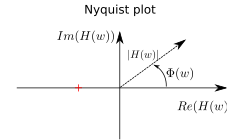
\includegraphics[width=.5\linewidth]{imgs/fourier/diagramme_nyquist}
        \end{center}
        \begin{block}{Definition}
          The Nyquist plot is a parametric plot of  $\tilde H(w)$ with 
        $Real(\tilde H(w))$ on x-axis and  $Imag(\tilde \Phi(w))$ on y-axis.
        \begin{itemize}
          \item Show the trajectory of $\tilde H$ in the complex plane.
          \item Used in system control to study the stability of systems.
        \end{itemize}
        \end{block}


        \frametitle{Frequency response of electronic systems}
 
\begin{block}{Principle}
  Ohm's law can be extended to capacitors and inductors using what is called complex called electrical impedance.
\end{block}
The linear system $i(t)\rightarrow u(t)$ is expressed as
$$\tilde U(w)=\tilde H(w)\tilde I(w)=\tilde Z(w)\tilde I(w)$$
\vspace{-5mm}
\begin{columns}[t]
  \begin{column}%{3cm}
    \begin{block}{Resistor}
      \begin{itemize}
      \item
$u(t)=Ri(t)$
\item \pause $\tilde U(w)=R\tilde I(w)$
\item $Z_R=R$
      \end{itemize}
    \end{block}
  \end{column}
  \begin{column}%{4cm}
    \begin{block}{Capacitor}
      \begin{itemize}
      \item
$u(t)=\frac{1}{C}\int_{-\infty}^ti(u)du$
\item \pause $\tilde U(w)=\frac{1}{jCw}\tilde I(w)$
%\item $U(w)=jLwI(w)$
\item $Z_C=\frac{1}{jCw}$
      \end{itemize}
    \end{block}
  \end{column}
  \begin{column}%{3.5cm}
    \begin{block}{Inductor}
      \begin{itemize}
      \item
$u(t)=L\frac{di(t)}{dt}$
\item \pause $\tilde U(w)=jLw\tilde I(w)$
\item $Z_L=jLw$
      \end{itemize}
    \end{block}
  \end{column}
\end{columns}
The frequency response of passive electronic systems can be computed with simple
computation of complex numbers.

\paragraph{First order system}

\begin{columns}
    \begin{column}%{6cm}
   \begin{itemize}
  \item System
\begin{align*}
x(t)&=Ri(t)+y(t)\\
y(t)&=\frac{1}{C}\int_{-\infty}^ti(v)dv \\
x(t)&=RCy'(t)+y(t)
\end{align*}
  \end{itemize}       
    \end{column}
    \begin{column}%{5cm}
      \begin{center}
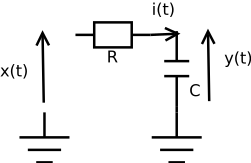
\includegraphics[width=.4\columnwidth]{imgs/fourier/RC2}
\end{center}
    \end{column}
  \end{columns}
  \begin{itemize}
  \item Frequency response\pause
$$ \tilde H(f)=\frac{Y(f)}{X(f)}={\frac{1}{1+RC2j\pi f}}$$
\item Using complex impedance\pause
\begin{equation*}
    \tilde Y(w)=Z_c \tilde I(w) \quad \text{ and } \quad \tilde X(w)= {(Z_R+Z_C) \tilde I(w)}
\end{equation*}
\begin{equation*}
    \tilde H(w)=\frac{ \tilde Y(w)}{\tilde \tilde X(w)}={\frac{Z_c}{Z_C+Z_R}=\frac{1}{1+\frac{Z_R}{Z_C}}=\frac{1}{1+RCjw}}
\end{equation*}
  \end{itemize}

  \begin{block}{Normalized system}
    We reformulate the frequency response as :
\begin{equation}
\label{eq:fobnctransfert_w0}
\tilde H(w)=\frac{1}{1+j\frac{w}{w_0}}
\end{equation}
where $w_0=\frac{1}{\tau}=\frac{1}{RC}$. 
  \end{block}
\textbf{Bode plot}
%\vspace{-5mm}
%\begin{columns}[t]
%\small
%    \begin{column}{6cm}
    \begin{block}{Modulus}\pause
\begin{enumerate}
\item $\tilde H(w)={\frac{1}{1+j\frac{w}{w_0}}}$
\item  $|\tilde H(w)|={\frac{1}{\sqrt{1+\frac{w^2}{w_0^2}}}}$
\item  $\tilde G(w)={20\log_{10}(|H(w)|)=-10\log_{10}(1+\frac{w^2}{w_0^2})}$
\item $\lim_{w\rightarrow 0}
\tilde G(w)={0}$
\item 
$\lim_{w\rightarrow\infty} \tilde G(w)={-10\log_{10}(\frac{w^2}{w_0^2})=-20\log_{10}(w)+20\log_{10}(w_0)}$
\item When $w=w_0$, $\tilde G(w)={-10\log_{10}(2)=-3dB}$
\end{enumerate}
    \end{block}

    \begin{block}{Argument}%\pause
        \begin{enumerate}
        \item $\tilde H(w)={\frac{1}{1+j\frac{w}{w_0}}}$
        \item $\tilde \Phi(w)={\arg(H(w))=-arg(1+jw)=-tan^{-1}(w)}$
        \item  $\lim_{w\rightarrow 0}
        \tilde  \Phi(w)={0}$
        \item   $\lim_{w\rightarrow\infty}\tilde \Phi(w)={-\pi/2}$
        \item  When $w=w_0$, $\tilde \Phi(w)={-tan^{-1}(1)=-\pi/4 \ (-45^\circ)}$
        
        when  $w=10w_0$,
          $\tilde \Phi(w)={-84^\circ}$
        
        when $w=.1w_0$
          $\tilde \Phi(w)={-6^\circ}$
        \end{enumerate}
              \end{block}

                \begin{block}{Bode plot}
                  \begin{center}
                    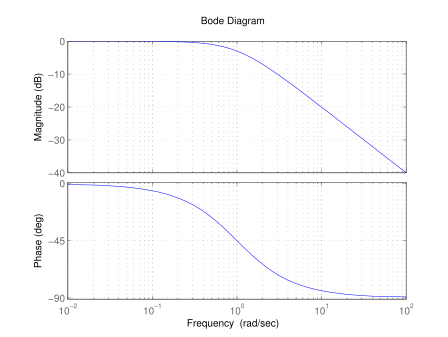
\includegraphics[width=.8\linewidth]{imgs/fourier/bode_rc}
                  \end{center}
                \end{block}

            

                    \begin{block}{Nichols plot}
                  \begin{center}
                    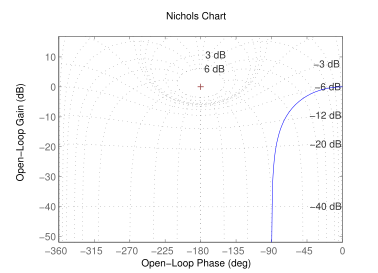
\includegraphics[width=.8\linewidth]{imgs/fourier/nichols_rc}
                  \end{center}
                \end{block}

            

                    \begin{block}{Nyquist plot}
                  \begin{center}
                    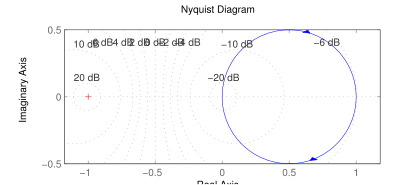
\includegraphics[width=.8\linewidth]{imgs/fourier/nyquist_rc}
                  \end{center}
                \end{block}

\paragraph{Secon order system}

\begin{columns}
    \begin{column}{6cm}
   \begin{itemize}
  \item Complex Impedance
\begin{align*}
\tilde Y(w)&=Z_c\tilde  I(w)\\
\tilde X(w)&= (Z_L+Z_R+Z_C) \tilde I(w)\\
\end{align*}
  \end{itemize}       
    \end{column}
    \begin{column}{5cm}
      \begin{center}
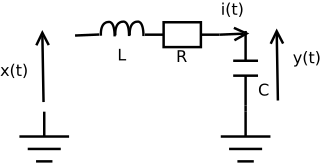
\includegraphics[width=.3\columnwidth]{imgs/fourier/RLC}
\end{center}
    \end{column}
  \end{columns}
  \begin{itemize}
  \item Frequency response
$$ \tilde H(w)=\frac{\tilde Y(w)}{\tilde X(w)}=\pause\frac{Z_C}{Z_L+Z_R+Z_C}=\frac{\frac{1}{jCw}}{\frac{1}{jCw}+R+jLw}$$
\item Normalized frequency response
\begin{equation*}
  \tilde H(w)=\frac{1}{1+RCjw+LC(jw)^2}=\frac{k}{1+2z\frac{jw}{w_n}+(\frac{jw}{w_n})^2}
\end{equation*}%\pause
\begin{itemize}
\item $k$ Static gain : $k=\pause{1}$
\item $z$ damping ratio of the system : $z=\pause {\frac{R}{2}\sqrt{\frac{C}{L}}}$
\item $w_n$ natural frequency of the system : $w_n=\pause {\frac{1}{\sqrt{LC}}}$
\end{itemize}
  \end{itemize}


  \begin{block}{Linear differential equation}
    The second order differential equation corresponding to the system is
        \begin{equation}
      \label{eq:syst_second_ordre}
      \frac{d^2y(t)}{dt^2}+2zw_n \frac{dy(t)}{dt}+w_n^2y(t)=kw_n^2x(t)
    \end{equation}
      \end{block}
      \begin{block}{Factorization}
    The second order system can be factorized as%\pause
    \begin{equation}
      \label{eq:transfsecondordre3}
      \tilde H(w)=\frac{kw_n^2}{(jw-c_1)(jw-c_2)}
    \end{equation}
    with
    
    \begin{align}
      \label{eq:6}
      c_1&={-zw_n+w_n\sqrt{z^2-1}}\\
      c_2&={-zw_n-w_n\sqrt{z^2-1}}
    \end{align}
     $c_1$ and $c_2$ are called the poles of the transfer function.
      \end{block}


      \begin{block}{Response of the system for  $z>1$}
        \begin{itemize}
        \item 
          $c_1$ and $c_2$ are real coefficients.
        \item The FT can be expressed as
          \begin{equation}
            \label{eq:transfsecondordre5}
            \tilde  H(w)=\frac{M}{jw-c_1}-\frac{M}{jw-c_2}
          \end{equation}
          with $M=\frac{w_n}{2\sqrt{z^2-1}}$,
        \item The impulse response of the system is
          \begin{equation*}
            h(t)=M(e^{c_1t}-e^{c_2t})\Gamma(t)
          \end{equation*}
    
        \item The step response of the system is
          \begin{equation*}
            e(t)=\left(1+M\left(\frac{e^{c_1t}}{c_1}-\frac{e^{c_2t}}{c_2}\right)\right)\Gamma(t)
          \end{equation*}
        \end{itemize}
    
      \end{block}


      \begin{block}{Response of the system for $z=1$}
        The FT becomes:
    \begin{equation}
      \label{eq:transfsecondordre3}
      \tilde H(w)=\frac{kw_n^2}{(jw+w_n)^2}
    \end{equation}
    that is the square of one first order system.
    
     The impulse response fo the system can be expressed as
    \begin{equation*}
      h(t)=w_n^2te^{-w_nt}\Gamma(t)
    \end{equation*}
    The step response can be expressed as
    \begin{equation*}
      e(t)=(1-e^{-w_nt}-w_nte^{-w_nt})\Gamma(t)
    \end{equation*}
      \end{block}


      \begin{block}{Response of the system for $z<1$}
        \begin{itemize}
        \item In this case the damping is weak and oscillations appear.
    \item This comes from teh fact that when
     $z<1$ coefficients $c_1$
     and $c_2$ are complex. The impulse response is
    \begin{equation*}
      h(t)=M(e^{c_1t}-e^{c_2t})\Gamma(t)
    \end{equation*}
    \item The step response is
    \begin{equation*}
      h(t)=\frac{w_ne^{-zw_nt}}{\sqrt{1-z^2}}\sin\left(w_nt\sqrt{1-z^2}\right)\Gamma(t)
    \end{equation*}
    that is  a sine with an exponentially decreasing magnitude. 
        \end{itemize}
     
    
    
    
      \end{block}


      \begin{block}{Impulse and step responses}
        \begin{center}
          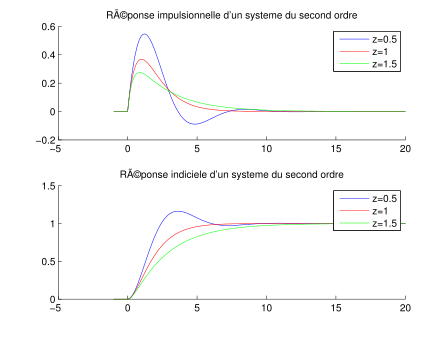
\includegraphics[width=10cm]{imgs/fourier/rep_2o}
        \end{center}
      \end{block}


      \begin{block}{Bode plot}
        We can plot the Bode plot using the normalized frequency response:
    \begin{equation}
      \label{eq:transfsecondordre2}
      H(w)=\frac{k}{\left(\frac{jw}{w_n}\right)^2+2z\left(\frac{jw}{w_n}\right)+1}
    \end{equation}
    \vspace{-5mm}
    \begin{block}{Modulus}
    \pause
    \small
      \begin{enumerate}
    \item $ \tilde  H(w)=\frac{k}{\left(\frac{jw}{w_n}\right)^2+2z\left(\frac{jw}{w_n}\right)+1}$.
    \item  $|\tilde H(w)|=\frac{k}{\sqrt{\left(1-\left(\frac{w}{w_n}\right)^2\right)^2+4z^2\left(\frac{w}{w_n}\right)^2}}$.
    \item  $\tilde G(w)=20\log_{10}(|\tilde H(w)|)=-10\log_{10}\left(\left(1-\left(\frac{w}{w_n}\right)^2\right)^2+4z^2\left(\frac{w}{w_n}\right)^2\right)+20log(k)$
    \item $\lim_{w\rightarrow 0}
    \tilde  G(w)=20log(k)$
    \item 
      $\lim_{w\rightarrow\infty} \tilde G(w)=-10\log_{10}(\frac{w^4}{w_n^4})=-40\log_{10}(w)+40\log_{10}(w_n)$
    \item En $w=w_0$, $\tilde G(w)=-20\log_{10}(2z)+20\log(k)$.
    \end{enumerate}
    \end{block}
      \end{block}

      \begin{block}{Properties of the modulus}
        \begin{itemize}
        \item The modulus of the frequency response for  $z<\sqrt(2)/2$ has a maximum at the following frequency
    \begin{equation*}
      w_{max}=w_n\sqrt{1-2z^2}
    \end{equation*}
    \item The value of the modulus at this frequency is
    \begin{equation*}
      |\tilde H(w_{max})|=\frac{k}{2z\sqrt{1-z^2}}
    \end{equation*}
    
    \item The cutoff frequency at -3dB is equal to
    \begin{equation*}
      w_{-3}=w_n\sqrt{1+2z^2+\sqrt{2-4z^2+4z^4}}
    \end{equation*}
    \end{itemize}
    
      \end{block}

      \textbf{Bode plot}
  \begin{block}{Argument}
\pause
\begin{enumerate}
\item $\tilde H(w)= \frac{k}{\left(\frac{jw}{w_n}\right)^2+2z\left(\frac{jw}{w_n}\right)+1}$.
\item $\tilde \Phi(w)=\arg(H(w))=-arg(\left(\frac{jw}{w_n}\right)^2+2z\left(\frac{jw}{w_n}\right)+1)=-tan^{-1}\left(\frac{2z\frac{w}{w_n}}{1-\frac{w^2}{w_n^2}}\right)$.
\item  $\lim_{w\rightarrow 0}
\tilde  \Phi(w)=0$
\item   $\lim_{w\rightarrow\infty}\tilde \Phi(w)=-\pi(-180^\circ )$
\item  En $w=w_0$, $\tilde \Phi(w)=-tan^{-1}(1)=-90^\circ$, 
\end{enumerate}

  \end{block}

  \begin{block}{Bode plot}
    \begin{center}
      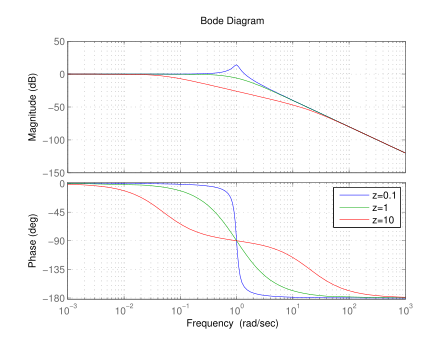
\includegraphics[width=.8\linewidth]{imgs/fourier/bode_2o}
    \end{center}
  \end{block}

  \begin{block}{Nichols plot}
    \begin{center}
      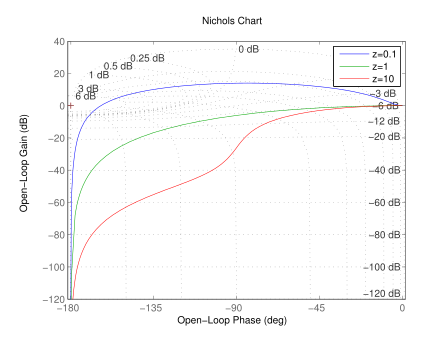
\includegraphics[width=.8\linewidth]{imgs/fourier/nichols_2o}
    \end{center}
  \end{block}

  \begin{block}{Nyquist plot}
    \begin{center}
      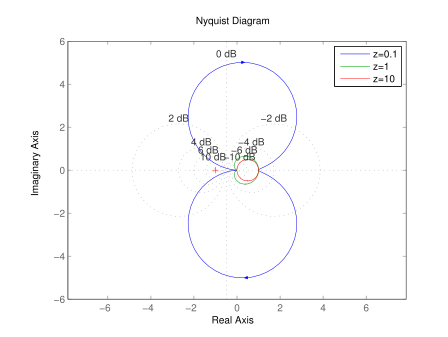
\includegraphics[width=.8\linewidth]{imgs/fourier/nyquist_2o}
    \end{center}
  \end{block}

%\lipsum[2-4]
\section{Applications of analog signal processing}
\label{sec:appli-ft}
%\lipsum[2-4]

\begin{block}{Applications of analog signal processing} \vspace{-1mm}
    \begin{itemize}
        \item Analog signal filtering. 
        \begin{itemize}
            \item Electronic passive and active filters.
            \item Modeling and filtering with physical systems.
        \end{itemize}
        \item Telecommunications. \vspace{-1mm}
            \begin{itemize}
                \item Amplitude modulation.
                \item Multiplexing.
            \end{itemize}
        \item Fourier opticsL\vspace{-1mm}
        \begin{itemize}
            \item Light propagation in perfect lens/mirror systems.
            \item Point spread functions of telescope and cameras.
        \end{itemize}
    \end{itemize}
\end{block}

\subsection{Analog filtering}
\label{sec:analogfiltering}

\subsubsection{Properties of analog filters}

\begin{block}{Definition}
    Signal processing system that aim at selecting part of the signal and attenuating another part (noise).

Analog filtering as opposed to digital filtering (next course)
  \end{block}


  \begin{block}{Objectives}
    \begin{itemize}
    \item Find a system that transform a signal $x(t)$ to extract pertinent information.
    \item Attenuate noise in a  signal.
    \item Separate several components of a signal (when different frequency bands).
    \end{itemize}
  \end{block}

  \frametitle{Filtering and bandwidth}

  \begin{block}{Gain and Attenuation}

    \begin{itemize}
    \item In order to characterize a filter one uses its 
    Gain/Phase (Bode plot).
$$\tilde G_{DB}(w)=20\log_{10}(|\tilde H(w)|)\quad \text{et}\quad
\tilde \Phi(w)=Arg(\tilde H(w))$$
     \item Attenuation is also often used $\tilde A(w)=-\tilde G_{DB}(w)$
 \end{itemize}
  \end{block}\vspace{-1mm}
  % \begin{block}{Synthèse de filtre}
  %   \begin{enumerate}
  %   \item Étudier le signal à filtrer (et le bruit).
  %   \end{enumerate}
  % \end{block}

  \begin{block}{Bandwith and passband}
   The band with of a filter is the set of frequency for which the Gain is over a reference
   (usually -3dB).
Bandwith at  $-3dB$:
\begin{equation*}
 BW= \left\{w|20\log\left(\frac{|\tilde H(w)|}{\max(|\tilde H(w)|)}\right)\geq-3\right\}
\end{equation*}
  \end{block} \vspace{-1mm}

  \begin{block}{Types of filters}\vspace{-2mm}
    \begin{itemize}
      \item \textbf{Low-pass},  $BW=[O,f_c]$ with $f_c$ cutoff frequency 
      \item \textbf{High-pass}, $BW=[f_c,\infty]$
      \item \textbf{Band-pass}, $BW=[f_{c_1},f_{c_2}]$
      \item \textbf{Band-stop}, $BW=[0,f_{c_1}]\cup [f_{c_2},\infty]$
    \end{itemize}
  \end{block}

  \frametitle{Filter distortion}
  
  \begin{block}{Undistorted transmission}
A signal is considered undistorted when the output of the system is
\vspace{3mm}
    \begin{columns}
      \begin{column}%{5.5cm}
        $$y(t)=Cx(t-t_0)$$
      \end{column}
      \begin{column}%{5.5cm}
With
\begin{itemize}
\item $C$ a constant gain.
\item $t_0>0$ is a delay. 
\end{itemize}

      \end{column}
    \end{columns}
  \vspace{3mm}


A system with no distortion has the following FT and impulse response
$$\tilde H(w)=\frac{\tilde X(w)}{\tilde Y(w)}=%\pause 
{Ce^{-jwt_0}} \quad \text{et} \quad
h(t)=%\pause 
{C\delta(t-t_0)}$$
With
\begin{itemize}
\item $|\tilde H(w)|=C$ or else amplitude distortion.
\item $Arg(\tilde H(w))=-wt_0$ or else phase distortion.
\end{itemize}
Note that the argument of the frequency response varies linearly with the frequency.
  \end{block}


  \begin{center}
    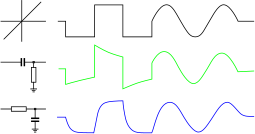
\includegraphics[width=.4\linewidth]{imgs/fourier/distortion.pdf}
  \end{center}
  
  \begin{block}{Phase distortion}
    Let a system of frequency response 
    $$\tilde H(w)=|H(w)|e^{j\phi(w)}$$

  We can deduce that for 
\begin{align*}
x(t)&=\cos(\omega t)\\
y(t)&=|\tilde H(\omega)| \cos(\omega t+ \phi(\omega))=|\tilde H(\omega)| \cos(\omega (t+ \phi(\omega)/\omega))
\end{align*}
The delay $\phi(\omega)/\omega$ is also called  \textbf{propagation time} of \textbf{frequency delay}.  For it to be independent from frequency it is necessary that
\begin{displaymath}
\frac{\phi(\omega)}{\omega}=cte=\tau\quad \rightarrow \quad \phi(\omega)=\omega\tau
\end{displaymath}
  \end{block}

  \frametitle{Ideal low pass filter}

  \begin{block}{Definition}
    \begin{itemize}
    \item The ideal low-pass filter is often a theoretical object in signal processing.
    \item Perfect to use when the noise and signal have non-overlapping spectra.
    \item The frequency response of the ideal filter is 
$$
H(f)= \left \{ 
\begin{array}{ll}
1 & \text{ if } |f| < f_c \\
0 & \text{ else} 
\end{array}
\right.
$$
where $f_c$ is the cutoff frequency.
\item The impulse response of the filter is %\pause
\begin{equation*}
  h(t)={2f_c\frac{\sin(2\pi f_c t)}{2\pi f_ct}=2f_c\text{sinc}(2\pi f_ct)}
\end{equation*}
    \end{itemize}
  \end{block}
\vspace{-5mm}
  \begin{block}{Realizable filter}
    \begin{itemize}
    \item A realizable temporal filter is \textbf{causal} and \textbf{stable} (absolute integrable).
    \item Ideal filter is neither of those and cannot be used for 1D (time) filtering.
    \item For images (2D) causality is not necessary.
    \end{itemize}
  \end{block}

\subsubsection{Filter design}
  
  \begin{block}{Real filter}
    \begin{itemize}
    \item Ideal filters are non causal and cannot be implemented in practice .
    \item We search for an approximation of the ideal filter.
    \item the approximation has to respect \textbf{constraints} (Gabarit in french).
    \end{itemize}
  \end{block}


  \begin{block}{Constraints of a filter}

\begin{columns}[T]
  \begin{column}%{5cm}
%\vspace{-5mm}
       \begin{center}
 % \includegraphics[width=1.1\columnwidth]{imgs/gabarit3}
 \begin{center}
  \includegraphics[width=.5\linewidth]{imgs/fourier/gabarit3}
\end{center}
\end{center}
  \end{column}%\vspace{-5mm}
  \begin{column}%{6cm}%\vspace{-5mm}
    \begin{block}{Parameters:}
      \begin{itemize}
      \item Bandwidth $BW$ and rejected band:
      \begin{itemize}
        \item $w_c$ cutoff frequency
        \item  $w_a$ attenuation frequency
      \end{itemize}
      \item Oscillations :
        \begin{itemize}
        \item $\varepsilon$ in passing bandwidth
        \item $\delta$ in attenuated bandwidth
        \end{itemize}
      \end{itemize}\vspace{7mm}
    \end{block}

  \end{column}
\end{columns}
 The constraints define the transfer function area that are acceptable for a given application.
  \end{block}

  \frametitle{Simple example  of filter design}
  \begin{columns}
  \begin{column}
 \begin{itemize}
\item Application to Brain computer interface.
\item Interesting signal for event related potentials below $\approx 12$Hz ($w_s=2\pi*12$).
\item Electrical noise (EDF) at $50$Hz ($w_{edf}=2\pi*50$).
\item Two low power signals $A_s\approx A_n$.
\item Maximum attenuation of signal at -3dB.
\item Filtering with first order filter.
\end{itemize}       
  \end{column}
  \begin{column}{5cm}
    \begin{center}
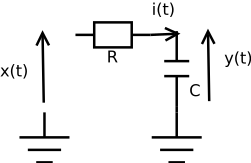
\includegraphics[width=.4\columnwidth]{imgs/fourier/RC2}
\end{center}
  \end{column}
\end{columns}

  \begin{columns}[t]
  \begin{column}
 \begin{itemize}
\item Frequency response
\pause
$$
\tilde H(w)=\frac{1}{1+j\frac{w}{w_0}}
$$
\item Gain in Db
\begin{equation*}
\tilde G(w)={-10\log_{10}\left(1+\frac{w^2}{w_0^2}\right)}
\end{equation*}
 \end{itemize}
  \end{column}
\begin{column}
  \begin{itemize}
  \item Before filtering:
    SNR$=20\log_{10}\left(\frac{A_s}{A_n}\right)=\pause
      {0}$
  \item After filtering : 

SNR$=\pause G(w_s)-G(w_{edf})$

\item Choice of $w_0$?
  \end{itemize}
  \end{column}
\end{columns}

\begin{itemize}
  \item SNR$=\tilde G(w_s)-\tilde G(w_{edf})$
  \item SNR is a decreasing function of $w_0$ .
  \end{itemize}     

  \paragraph{What is the best value for $w_0$?}
  
  \begin{itemize}
    \item With the maximum attenuation of 3dB constraint.
      $\rightarrow \pause w_s\leq w_0 \leq \infty$.
    \item For $w_0=w_{edf}\rightarrow R_{S/B}=\pause {2.76 dB}$ 
    \item For $w_0=(w_{edf}+w_s)/2={37*2*\pi}\rightarrow
      R_{S/B}=\pause {4.07dB}$
    \item Pour $w_0=w_{s}\rightarrow R_{S/B}=\pause {9.63dB}$ 
    \end{itemize}
     $\rightarrow w_0=w_s$ respects the constraint and maximizes the SNR.


     \frametitle{Approximating a low pass filter }

     \begin{center}
       
\includegraphics[width=.45\columnwidth]{imgs/fourier/gabarit1}
    \includegraphics[width=.45\columnwidth]{imgs/fourier/gabarit2}
     \end{center}
   
     \begin{block}{Constraints for a low-pass filter}
       \begin{itemize}
       \item Passband: 
   $ 1-\varepsilon \leq |\tilde H(w)| \leq 1 \quad \text{pour} \quad w<w_p$
   \begin{itemize}
   \item $w_p$: passing frequency.
   \item $\varepsilon$: passband margin parameter ($\varepsilon=1/2\rightarrow-3dB$).
   \end{itemize}
   \item Stopband : $ |\tilde H(w)| \leq \delta \quad \text{pour} \quad w>w_a$
     \begin{itemize}
   \item $w_a$: attenuation frequency.
   \item $\delta$: stopband margin parameter.
     \end{itemize}
   \item $w_a-w_c$ is the transition band.
       \end{itemize}
     \end{block}

     \paragraph{Additional constraints}
     
     \begin{itemize}
      \item Need for an approximation function that respects the constraints \emph{constrained optimization}.
      \item Criterion is optimized (for instance maximization of SNR).
      \item Two approaches are usually used:
      \end{itemize}
    
      \begin{block}{Maximally flat frequency response}
        \begin{itemize}
          \item Minimal distortion is achieved when the passband is flat.
        \item Let $|\tilde H(w)|$ be the modulus of the frequency response of an order $k$ filter.
      \item  $|\tilde H(w)|$ is \textit{maximally flat} in 
        $w=0$ if all the $K^{th}$derivatives are null
        \end{itemize}
    $$\frac{d^K|\tilde H(w)|}{dw^K}=0$$
      \end{block}
      \begin{block}{Equiripple filter}
        \begin{itemize}
          \item A better rollof (sharper decrease) can be achieved at teh cost of oscillations.
          \item Oscilations can occur in the passband (leading to distortion) of cutband (limited attenuation).
          %\item  On can accept some oscillations in the passband in order to get sharp decrease (roll-off).
          \item An equiripple filter has constant magnitude for its oscillations in the bandpass.
        \end{itemize}
        %%One an  accept some socillation in the passband in order to get sharp decrease. An equiripple filter has constant magnitude for its oscillations in the bandpass.
      \end{block}

\subsubsection{Classical Analog Filters}

\paragraph{Butterworth filter}

\begin{itemize}
  \item  Butterworth filters are  \emph{maximally
    flat} \cite{butterworth1930theory}.
\item The amplitude of the frequency response can be expressed as
  \begin{columns}
        \begin{column}{6cm}
    \begin{equation}
      \label{eq:a_butter}
      |\tilde H(w)|=\frac{1}{\sqrt{1+\left(\frac{w}{w_c}\right)^{2n}}}
    \end{equation}
    with
    \begin{itemize}
    \item $n$: order of the filter.
    \item $w_c$: cutoff frequency.
    \end{itemize}
  \end{column}
  \begin{column}{4cm}
    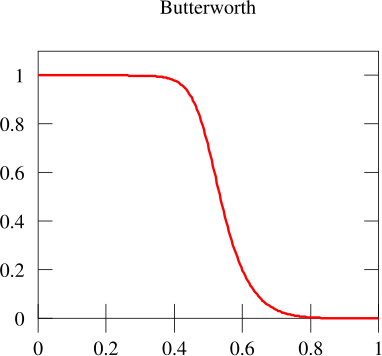
\includegraphics[width=.5\columnwidth]{imgs/fourier/butterworth}
  \end{column}
  \end{columns}
\item The passing $w_p$ and
  attenuation $w_a$ frequencies  are:
\vspace{.5cm}
\begin{columns}
     \begin{column}{5.5cm}
For $|\tilde H(w)|=1-\varepsilon$
   $$w_p=\pause{ w_c\left(\frac{\varepsilon}{1-\varepsilon}\right)^{1/2n}}$$
  \end{column}
  \begin{column}{5.5cm}
For $|\tilde H(w)|=\delta$
$$w_a=\pause {w_c\left(\frac{1-\delta}{\delta}\right)^{1/2n}}$$
  \end{column}
  \end{columns}

  \end{itemize}

  \begin{itemize}
    \item The Butterworth filter is monotonically decreasing with the frequency.
    \item The amplitude of the frequency response can be expressed as
$$|\tilde H(w)|=1-\frac{1}{2}\left(\frac{w}{w_c}\right)^{2n}+\frac{3}{8}\left(\frac{w}{w_c}\right)^{4n}-\frac{5}{16}\left(\frac{w}{w_c}\right)^{6n}+\dots$$
\item The derivative in $w=0$ is then null up to order 
  $k=\pause 2n-1$.
\item The frequency response of a (normalized) Butterworth filter can be expressed as $\tilde H(w)  =\frac{1}{B_n(w)}$ where  $B_n(w)$ is a Butterworth polynomial :
\begin{equation*}\footnotesize
, \quad B_n(w)= \begin{cases} \prod_{k=1}^{\frac{n}{2}} \left[(jw))^2-2jw\cos\left(\frac{2k+n-1}{2n}\,\pi\right)+1\right] &\mbox{if } n =  \text{ even} \\
  (jw+1)\prod_{k=1}^{\frac{n-1}{2}} \left[(jw))^2-2jw\cos\left(\frac{2k+n-1}{2n}\,\pi\right)+1\right] & \mbox{if } n =  \text{ odd}  \end{cases}
\end{equation*}
%where
\begin{columns}[T]
  \begin{column}
    \begin{tabular}{|c|c|}\hline
      Order & Polynomial \\\hline
      1 & $1+jw$\\
      2 & $(jw)^2+\sqrt{2}jw+1$\\
      3& $(jw+1)((jw)^2+jw+1)$ \\\hline
    %  4& $((jw)^2+0.7654jw+1)((jw)^2+1.8478jw+1)$ \\\hline
    \end{tabular}
  \end{column}
\end{columns}
\begin{center}

 
\end{center}
    \end{itemize}

\paragraph{Chebyshev filter}



\begin{center}
  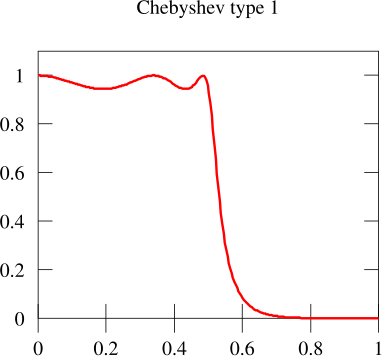
\includegraphics[width=.35\columnwidth]{imgs/fourier/cheby1}\hspace{1cm}
  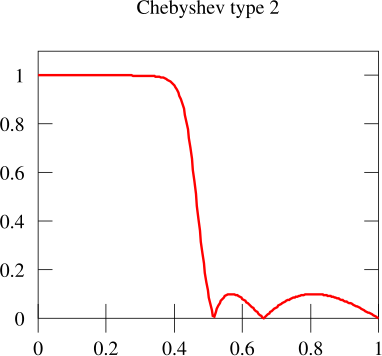
\includegraphics[width=.35\columnwidth]{imgs/fourier/cheby2}
\end{center}
\begin{itemize}
\item Better rolloff than Butterworth of same order but leads to oscillations in the bandpass (type 1) or in the stopband (type 2).
\item \emph{Equiripple} filter.
\item Amplitude of the frequency response:
 \begin{columns}
   \begin{column}{6cm}
$$  |\tilde H(w)|=\frac{1}{\sqrt{1+\varepsilon^2T_n^2\left(\frac{w}{w_c}\right)}}$$
\end{column}
\begin{column}{5cm}
\begin{itemize}
\item $T_n(\cdot)$: Chebyshev polynomial of order $n$.
\end{itemize}
\end{column}
\end{columns}

\end{itemize}
    

\subsection{Filter implementation}

 Implementation of the filter consist in finding the physical components that recovers the selected  frequency response $\tilde H(w)$.


  \begin{block}{Passive filter}
    \begin{itemize}
    \item Only passive components (R, C, L).
   % \item Utilisation de condensateur, bobine , résistance.
    \item No energy source, no amplification (conservation of energy).
    \item The input and output impedance has an effect on the frequency response (impedance matching).
    \end{itemize}
  \end{block}

  \begin{block}{Active filter}
       \begin{itemize}
    \item Use an energy source and Operational Amplifiers (OA).
    %\item No need for impedance matching.
   % \item Slightly more expensive.
    %\item Mise en oeuvre à l'aide d'amplificateur opérationnel (AOP).
    \item OA has near infinite impedance  but limited bandwidth (typically 100KHz).
    \item Saturation can occur (non-linearity).
    \item Stability can be a problem (due to feedback)
  %  \item 
    \end{itemize}
  \end{block}
  Rarely use inductors in practice (price, resistance, space, mutual inductance) !

\paragraph{Passive filters}

\begin{block}{Example filter}
  \begin{columns}
\begin{column}{7cm}
\begin{itemize}
\item Brain-Computer Interface application.
\item $w_0=w_s=2\pi*12$
\item $w_0=\frac{1}{RC}\rightarrow RC={\frac{1}{2*\pi*12}\approx 0.01326}$
\item What to choose for $R$ and $C$ ?
\item Price and space constraints.
\end{itemize}     
\end{column}
\begin{column}{5cm}
\begin{center}
\includegraphics[width=.5\columnwidth]{imgs/fourier/RC2}
\end{center}
\end{column}
\end{columns}
\end{block}
\begin{block}{Filter transformation}
\begin{itemize}
%  \item Transformation similaire à celle effectuée sur les FT.
\item \textbf{low-pass $\rightarrow$ high-pass}
$$ 1/jCw\rightarrow jLw \quad  \text{et} \quad jLw \rightarrow 1/jCw$$
\item \textbf{low pass $\rightarrow$ band-pass}
$$ 1/jCw\rightarrow B/C(jw+1/jw) \quad  \text{et} \quad jLw \rightarrow L/B/(jw+1/jw)$$
\end{itemize}
\end{block}

\begin{block}{Butterworth Filter}
  \begin{itemize}
  \item Corresponding frequency response with the Cauer topology.
  \item For an order $n$ filter with cutoff frequency $w_c=1$ the following structure:
   \begin{center}
\includegraphics[width=.8\columnwidth]{imgs/fourier/Cauer_lowpass}
\end{center}
With the values :
\begin{itemize}
\item $C_k=2\sin(\frac{2k-1}{2n}\pi)$ for $k$ odd.
\item $L_k=2\sin(\frac{2k-1}{2n}\pi)$ for $k$ even.
\end{itemize}
\item Assuming the input and output have a $1$ Ohm resistance.
\end{itemize}
\end{block}

\paragraph{Active filters}

\begin{block}{First order active filter (with amplification)}

  \begin{center}
\includegraphics[width=6cm]{imgs/fourier/filtrage_actif_1o}

\begin{itemize}
\item Frequency response
$$\tilde H(w)=\frac{A}{1+\frac{jw}{w_0}}$$
where 
$$A=\pause {\frac{R_1+R_2}{R_1}} \quad \text{et} \quad  w_0= \pause {\frac{1}{RC}}$$

\item Parameters: $R, C,R_1,R_2$
\item  Permute $R$ and $C$ for a high-pass filter.
\end{itemize}
\end{center}
\end{block}

\begin{block}{Second order active filter (Structure from \cite{sallen1955practical}) }
\vspace{-5mm}
  \begin{center}
\includegraphics[width=.8\columnwidth]{imgs/fourier/filtrage_actif_2o}
\end{center}
\vspace{-5mm}
\begin{itemize}
\item Frequency response
$$\tilde H(w)=\frac{K}{1+\frac{2zjw}{w_n}+\frac{(jw)^2}{w_n^2}}$$\vspace{-5mm}
where \pause
$$ w_n=\frac{1}{R\sqrt{C_1C_2}}\quad \text{et} \quad
z=\sqrt{\frac{C_1}{C_2}} \frac{3-K}{2}\quad \text{et} \quad  K=\frac{r_1+r_2}{r_1}$$

\item Parameters: $R, C_1,C_2,r_1,r_2$.

\end{itemize}
\end{block}

\frametitle{Analog filtering : mechanical filter}


\begin{columns}[T]
  \begin{column}
    \begin{block}{Virgo Gravitational waves detector \cite{acernese2014advanced}}
      \begin{itemize}
        \item Interferometer to detect gravitational waves.
        \item Attenuate vibrations from the earth \cite{braccini1996seismic}
        \item Objective : attenuations of $10^{-9}$ for high frequencies. 
        \item Use a mirror in  a chamber with mechanical filters.
        \item Use a series of mechanical filters for the attenuation.
        \item Active correction for remaining low frequencies.
      \end{itemize}
    \end{block}
  \end{column}\hspace{-1cm}

\end{columns}


\begin{center}
  \includegraphics[width=.2\linewidth]{imgs/fourier/virgo_mechanical_filter.png}
  \includegraphics[width=.75\linewidth]{imgs/fourier/virgo_mechanical_filter_response.png}
\end{center}


\subsection{Modulation}
\label{sec:modulation}

\frametitle{Modulation}
  

%\begin{block}{Definition}
  Modulation is an encoding method that allows to transport a band-limited signal.
  Demodulation is the reverse operation.
%\end{block}
\begin{exampleblock}{Motivations}
  \begin{itemize}
  \item Raw signal transmission often not efficient
    (electromagnetic waves).
%  \item Signal à transmettre de bande passante finie.
  \item The change in frequencies allow transmitting several band-limited signals in parallel.
  \item Use only of an authorized bandwidth.
  \end{itemize}
\end{exampleblock}

\begin{block}{Definitions}
\begin{itemize}
  \item \textbf{Modulating signal} $x(t)$ is a band limited signal we want to transmit ($ X(f)=0\quad \text{pour}\quad |f|>f_x$).
  \item \textbf{Carrier} is the periodic base signal $p(t)$ used for transportation often : $$ p(t)= \cos(2\pi f_p t)$$
  \item \textbf{Modulated signal} $y(t)$ is a band-limited signal that can be transported in the physical medium (cable, air, optical fiber)
\end{itemize}
\end{block}

\subsubsection{Amplitude modulation}

\begin{columns}
  \begin{column}{5cm}\centering
     \includegraphics[width=.45\linewidth]{imgs/fourier/modul_amplitude}
  \end{column}
  \begin{column}{5cm}
\includegraphics[width=.45\linewidth]{imgs/fourier/illustration_mod_ampl.pdf}
     % \includegraphics[width=.9\linewidth]{imgs/mod_porteuse}\\
     % \includegraphics[width=.9\linewidth]{imgs/mod_modulant}\\
     % \includegraphics[width=.9\linewidth]{imgs/mod_module}
  \end{column}
\end{columns}
 

\begin{block}{Definition: Amplitude Modulation (AM)}
The carrier is multiplied by the modulating signal  $x(t)$ 
  \begin{equation*}
y(t)=A_c(1+k_sx(t))\cos(2\pi f_p t+\phi_m)
\end{equation*}
\vspace{-5mm}
\begin{itemize}
\item $k_s$: modulation factor
\item $f_p$: carrier frequency
\item $\phi_m$: phase (usually added during transmission).
\end{itemize}
\end{block}



\begin{columns}
  \begin{column}{6cm}

     \begin{block}{Modulation index}
       \begin{itemize}
       \item  Envelope of the modulated signal.
$$a(t)=A_c|1+k_sx(t)|$$
       \item Maximum amplitude of modulating signal:

$$M_x=\max_t|x(t)|$$
       \item The index of modulation is defined as 
$$h=k_sM_x$$
\vspace{-5mm}
\begin{itemize}
\item $h<1$: under-modulation.
\item $h>1$: over-modulation.
\end{itemize}

       \end{itemize}
 
\end{block}
\end{column}
  \begin{column}{4.5cm}
%\hspace{-1cm}
      \includegraphics[width=0.5\linewidth]{imgs/fourier/mod_ampl_h.pdf}

  \end{column}
\end{columns}

\begin{block}{Interpretation in the Fourier domain}
  \begin{columns}
  \begin{column}{5.5cm}
    \begin{itemize}
    \item Multiplication $\rightarrow$ Convolution.
$$Y(f)=X(f)\star P(f)$$
    \item The spectrum of the modulating signal is moved around the frequency $f_p$.
    \item Simple way to transmit a band limited signal in a given bandwidth.
    \item Modulated signal spectrum is contained in $f_p\pm f_x$.
    \end{itemize}
  \end{column}\hspace{-5mm}
  \begin{column}{5.5cm}
    \begin{center}\vspace{-1cm}\hspace{-5mm}
      \includegraphics[width=0.5\linewidth]{imgs/fourier/mod_ampl_spectrum2.pdf}
    \end{center}

  \end{column}        
  \end{columns}

\end{block}

\begin{block}{Synchronous demodulation}
  Done with multiplying the signal with the carrier:
\begin{align*}
\label{eq:4}
w(t)&=y(t)\cos(2\pi f_p t+\phi_d)\\
&=A_s(1+k_sx(t))\cos(2\pi f_p t+\phi_m)\cos(2\pi f_p t+\phi_d)\\
&={{\frac{A_s}{2}(1+k_sx(t))\cos(\phi_m-\phi_d)+\frac{A_s}{2}(1+k_sx(t))\cos(4\pi f_pt+\phi_m+\phi_d)}}
\end{align*}%\pause
After low pass filtering (and removing of the constant) one can recover 
$$\hat x(t)=\frac{A_s}{2}k_sx(t)\cos(\phi_m-\phi_d)$$
\begin{itemize}
\item  $\cos(\phi_m-\phi_d)=1$ if $\phi_m=\phi_d$.
\item Very important to have a good synchronization (requires active components).
\end{itemize}
\end{block}


\begin{center}
\includegraphics[width=.2\linewidth]{imgs/fourier/demod_asynchrone}\hspace{1cm}
\includegraphics[width=.5\linewidth]{imgs/fourier/demod_ampl_async.pdf}
\end{center}
\begin{block}{Asynchrone demodulation}
  \begin{itemize}
  \item Synchronous demodulation can require complex active components.
  \item A coarse approximation of the envelope of the signal can be done with a  simple diode/RC system.
  \item Requires under-modulation because if $h<1$ then
$$a(t)=A_c|1+k_sx(t)|=A_c+ A_ck_sx(t)$$
\item Can require a lot of power for transmission.
  \end{itemize}
\end{block}


\paragraph{Applications of AM}


\begin{center}
  \includegraphics[height=2.5cm]{imgs/fourier/Telefunken_arc_radiotelephone.jpg}
  \includegraphics[height=2.5cm]{imgs/fourier/triode.png}
  \includegraphics[height=2.5cm]{imgs/fourier/eiffel_antena.jpeg}
  \includegraphics[height=2.5cm]{imgs/fourier/Emetteur-allouis3.jpg}
\end{center}

\begin{block}{Low frequency radio broadcasting}\vspace{-2mm}
  \begin{itemize}
    \item First AM transmission R. Fessenden on 23 December 1900 at  Cobb Island, Maryland (1.6Km).
    \item 1907 Lee de Forest invents the triod vacuum tube allowing for a better amplification \cite{de1908space}.
    \item Weather bulletin emitted from the Eiffel Tower in february 1922. 
    \item \textbf{France Inter grandes ondes}
    \begin{itemize}
      \item Emitted between 1 January 1947 and 31 December 2016.
      \item Allouis longwave transmitter (2000KW), now used for TDF time signal.
    \end{itemize}
  \end{itemize}
\end{block}

\begin{center}
  \includegraphics[width=.65\linewidth]{imgs/fourier/illus_multiplex.pdf}
\end{center}
\vspace{-3mm}
 %   \begin{columns}[t]
  %    \begin{column}{6cm}
   \begin{block}{Frequency-division multiplexing}
        \begin{itemize}
        \item Multiplexing: transmission of several signals in parallel.
         \item Use of a different $f_p$ for each signal.
        \item Every signal is band limited : if $\Delta f_p>2f_x$ then no loss of information.
        
      %  \item If $\Delta f_p>2f_x$ then no loss of information.
        \item Frequency Hoping: Experimented by G. Marconi, Patent by N. Tesla \cite{tesla1903system}, proposed for secret communication by \cite{kiesler1942secret}.
        \end{itemize}
    \end{block}

\subsubsection{Frequency modulation}

\begin{center}
  \includegraphics[width=.8\linewidth,height=2.5cm]{imgs/fourier/illustration_mod_frq.pdf}
\end{center}
\vspace{-5mm}
    \begin{block}{Definition}
      Frequency modulation (FM) consists in modifying the frequency of the carrier using $x(t)$. 
      The modulated signal has the following form:
\begin{equation*}
  y(t)=\cos\left(2\pi  \int_0^tf(\tau)d\tau\right)
\end{equation*}
\vspace{-.5cm}
\begin{itemize}
\item $f(t)= f_p+  f_\Delta x(t)$ is the instantaneous frequency of the signal.
  \begin{itemize}
  \item If $x(t)=0$ we recover the carrier.
  \item When $x(t)\neq 0$ the instantaneous frequency is modified by $x(t)$
  \end{itemize}
\item $f_\Delta$ is the frequency deviation (equivalent to $k_s$ in
  AM).

\end{itemize}
    \end{block}

    \begin{block}{Properties of Frequency Modulation}
      \begin{itemize}
\item More robust than AM (noise, atténuation) but propagation distance limited.
\item More complex to implement (requires a Voltage Controled
Oscillator VCO).
\item Intuitively the spectrum of the modulated signal should be $\neq 0$
only in the band $f_p\pm f_\Delta M_x$, BUT
\item Continuous variation of the frequencies imply a spectrum on all frequencies.
\item The Carson bandwidth rule states that most of the signal power (98\%) is in the band 
\begin{equation*}
  b=2(f_\Delta+f_{x})
\end{equation*}
%\item Cours de modulation en M1.
      \end{itemize}
    \end{block}

    \begin{block}{Application of Frequency Modulation}
      \begin{itemize}
        \item FM radio broadcasting.
        \item Frequency modulation synthesis (chiptunes).
        \item Magnetic tape storage. 
      \end{itemize}
    \end{block}

\subsection{Fourier optics}
\label{sec:}

\chapter{Digital signal processing}
\label{chap:dsp}


\section{Sampling and Analog/Digital conversion}
\label{sec:sampling}

\section{Digital filtering and transfer function}
\label{sec:digital_filtering}

\section{Finite signals and Fast Fourier Transform}
\label{sec:finite_signals_fft}

\section{Applications of DSP}
\label{sec:applis_dsp}

\chapter{Random signals}
\label{chap:random}


\section{Random Signals and Correlations}
\label{sec:rand_sig_corr}

\section{Frequency representation of random signals}
\label{sec:freq_resp_random}

\section{AR modeling and linear prediction}
\label{sec:ar_linear}

\chapter{Signal representations}
\label{chap:sig_representations}

\section{Short Time Fourier Transform}
\label{sec:stft}

\section{Common signal representations}
\label{sec:comon_signal_rep}

\section{Source separation and dictionary learning}
\label{sec:dl}


\section{Machine learning for signal processing}
\label{sec:mlsp}


%\ForceHTMLTOC 
\ForceHTMLPage

\bibliographystyle{apalike}
\bibliography{biblio}
\addcontentsline{toc}{chapter}{Bibliography}
% \begin{warpprint}
%     \addcontentsline{toc}{chapter}{Bibliography}
% \end{warpprint}

\ForceHTMLPage
\printindex
\addcontentsline{toc}{chapter}{Index}
\begin{warpprint}
% \ForceHTMLPage
\listoftheorems[title={List of definitions},ignoreall,show={definition},onlynamed={definition}]
\addcontentsline{toc}{chapter}{List of definitions}
\end{warpprint}
\end{document}